\documentclass[14pt]{beamer}
\usetheme{zdr}
%
\usepackage{booktabs} % \toprule, etc
% My macros
% Zach del Rosario's LaTeX macros (zdelrosario@outlook.com)
% Inspired by Paul Constantine, Art Owen
% Thanks to David Carlisle for writing the numdef package,
%    which makes the fraction definitions possible!

% Use % Zach del Rosario's LaTeX macros (zdelrosario@outlook.com)
% Inspired by Paul Constantine, Art Owen
% Thanks to David Carlisle for writing the numdef package,
%    which makes the fraction definitions possible!

% Use % Zach del Rosario's LaTeX macros (zdelrosario@outlook.com)
% Inspired by Paul Constantine, Art Owen
% Thanks to David Carlisle for writing the numdef package,
%    which makes the fraction definitions possible!

% Use \input{zachs_macros} in preamble of a latex document

% --------------------------------------------------
% Use some package dependencies
% --------------------------------------------------
\usepackage{amsmath}  % for \boldsymbol, etc.
\usepackage{amsfonts} % for \mathbb, etc.
\usepackage{scalerel,stackengine} % for \reallywidehat{}
\usepackage{graphicx} % for \includegraphics
\usepackage{caption}  % for captioning
\usepackage{mathtools}% for \ceil and \floor
\usepackage{forest}   % for forest environment

% --------------------------------------------------
% Figures and tables
% --------------------------------------------------
% Could use as-is; better for pattern matching

% Image Macro: \img{filename}{caption}
\newcommand{\img}[2]{
	\begin{figure}[H]
	\centering
	\includegraphics[width=0.6\textwidth]{../images/#1}   % first argument is the file
	\caption{#2}                  % second argument is caption
	\label{fig:#1}                % generate label from first argument
	\end{figure} }

% Double Image Macro: \img{file1}{file2}{caption1}{caption2}
\newcommand{\imgtwo}[4]{
	\begin{figure}
	\centering
	\begin{minipage}{.5\textwidth}
		\centering
		\includegraphics[width=0.9\linewidth]{../images/#1}
		\captionof{figure}{#3}
		\label{fig:#1}
	\end{minipage}%
	\begin{minipage}{.5\textwidth}
		\centering
		\includegraphics[width=0.9\linewidth]{../images/#2}
		\captionof{figure}{#4}
		\label{fig:#2}
	\end{minipage}
	\end{figure}
}

% Table Macro: \tab{filename}{caption}
\newcommand{\tab}[2]{
	\begin{table}[H]
	\centering
	\input{#1} 	% first argument is filename
	\caption{#2} 			% second argument is caption
	\label{tab:#1} 			% generate label from filename
	\end{table}
}

% --------------------------------------------------
% Common sets
% --------------------------------------------------
% Lovingly ripped from Art Owen
\def\reals{\mathbb{R}} % Real number symbol
\def\integers{\mathbb{Z}} % Integer symbol
\def\rationals{\mathbb{Q}} % Rational numbers
\def\naturals{\mathbb{N}} % Natural numbers
\def\complex{\mathbb{C}} % Complex numbers
% With exponent
\def\R#1{\mathbb{R}^{#1}}
\def\Z#1{\mathbb{Z}^{#1}}
\def\Q#1{\mathbb{Q}^{#1}}
\def\N#1{\mathbb{N}^{#1}}
\def\C#1{\mathbb{C}^{#1}}

% --------------------------------------------------
% Vectors and Matrices
% --------------------------------------------------
% Transpose symbol
\newcommand{\T}{\top}
% Vector symbol macros
\newcommand{\vsym}[1]{\boldsymbol{#1}}
\def\v#1{\vsym{#1}} % \v{x} for vector symbol
% Quick letter vectors
\newcommand{\va}{\boldsymbol{a}}
\newcommand{\vb}{\boldsymbol{b}}
\newcommand{\vc}{\boldsymbol{c}}
\newcommand{\vd}{\boldsymbol{d}}
\newcommand{\ve}{\boldsymbol{e}}
\newcommand{\vf}{\boldsymbol{f}}
\newcommand{\vg}{\boldsymbol{g}}
\newcommand{\vh}{\boldsymbol{h}}
\newcommand{\vi}{\boldsymbol{i}}
\newcommand{\vj}{\boldsymbol{j}}
\newcommand{\vk}{\boldsymbol{k}}
\newcommand{\vl}{\boldsymbol{l}}
\newcommand{\vm}{\boldsymbol{m}}
\newcommand{\vn}{\boldsymbol{n}}
\newcommand{\vo}{\boldsymbol{o}}
\newcommand{\vp}{\boldsymbol{p}}
\newcommand{\vq}{\boldsymbol{q}}
\newcommand{\vr}{\boldsymbol{r}}
\newcommand{\vs}{\boldsymbol{s}}
\newcommand{\vt}{\boldsymbol{t}}
\newcommand{\vu}{\boldsymbol{u}}
\newcommand{\vv}{\boldsymbol{v}}
\newcommand{\vw}{\boldsymbol{w}}
\newcommand{\vx}{\boldsymbol{x}}
\newcommand{\vy}{\boldsymbol{y}}
\newcommand{\vz}{\boldsymbol{z}}

% Tilde shortcut
\newcommand{\tl}[1]{\tilde{#1}}
% Vector symbol + tilde macros
\newcommand{\vta}{\tilde{\boldsymbol{a}}}
\newcommand{\vtb}{\tilde{\boldsymbol{b}}}
\newcommand{\vtc}{\tilde{\boldsymbol{c}}}
\newcommand{\vtd}{\tilde{\boldsymbol{d}}}
\newcommand{\vte}{\tilde{\boldsymbol{e}}}
\newcommand{\vtf}{\tilde{\boldsymbol{f}}}
\newcommand{\vtg}{\tilde{\boldsymbol{g}}}
\newcommand{\vth}{\tilde{\boldsymbol{h}}}
\newcommand{\vti}{\tilde{\boldsymbol{i}}}
\newcommand{\vtj}{\tilde{\boldsymbol{j}}}
\newcommand{\vtk}{\tilde{\boldsymbol{k}}}
\newcommand{\vtl}{\tilde{\boldsymbol{l}}}
\newcommand{\vtm}{\tilde{\boldsymbol{m}}}
\newcommand{\vtn}{\tilde{\boldsymbol{n}}}
\newcommand{\vto}{\tilde{\boldsymbol{o}}}
\newcommand{\vtp}{\tilde{\boldsymbol{p}}}
\newcommand{\vtq}{\tilde{\boldsymbol{q}}}
\newcommand{\vtr}{\tilde{\boldsymbol{r}}}
\newcommand{\vts}{\tilde{\boldsymbol{s}}}
\newcommand{\vtt}{\tilde{\boldsymbol{t}}}
\newcommand{\vtu}{\tilde{\boldsymbol{u}}}
\newcommand{\vtv}{\tilde{\boldsymbol{v}}}
\newcommand{\vtw}{\tilde{\boldsymbol{w}}}
\newcommand{\vtx}{\tilde{\boldsymbol{x}}}
\newcommand{\vty}{\tilde{\boldsymbol{y}}}
\newcommand{\vtz}{\tilde{\boldsymbol{z}}}

% Vector symbol + hat macros
\newcommand{\vha}{\hat{\boldsymbol{a}}}
\newcommand{\vhb}{\hat{\boldsymbol{b}}}
\newcommand{\vhc}{\hat{\boldsymbol{c}}}
\newcommand{\vhd}{\hat{\boldsymbol{d}}}
\newcommand{\vhe}{\hat{\boldsymbol{e}}}
\newcommand{\vhf}{\hat{\boldsymbol{f}}}
\newcommand{\vhg}{\hat{\boldsymbol{g}}}
\newcommand{\vhh}{\hat{\boldsymbol{h}}}
\newcommand{\vhi}{\hat{\boldsymbol{i}}}
\newcommand{\vhj}{\hat{\boldsymbol{j}}}
\newcommand{\vhk}{\hat{\boldsymbol{k}}}
\newcommand{\vhl}{\hat{\boldsymbol{l}}}
\newcommand{\vhm}{\hat{\boldsymbol{m}}}
\newcommand{\vhn}{\hat{\boldsymbol{n}}}
\newcommand{\vho}{\hat{\boldsymbol{o}}}
\newcommand{\vhp}{\hat{\boldsymbol{p}}}
\newcommand{\vhq}{\hat{\boldsymbol{q}}}
\newcommand{\vhr}{\hat{\boldsymbol{r}}}
\newcommand{\vhs}{\hat{\boldsymbol{s}}}
\newcommand{\vht}{\hat{\boldsymbol{t}}}
\newcommand{\vhu}{\hat{\boldsymbol{u}}}
\newcommand{\vhv}{\hat{\boldsymbol{v}}}
\newcommand{\vhw}{\hat{\boldsymbol{w}}}
\newcommand{\vhx}{\hat{\boldsymbol{x}}}
\newcommand{\vhy}{\hat{\boldsymbol{y}}}
\newcommand{\vhz}{\hat{\boldsymbol{z}}}

% Matrix symbol
\newcommand{\msym}[1]{\boldsymbol{#1}}
\def\m#1{\msym{#1}} % short-shortcut

\newcommand{\mA}{\boldsymbol{A}}
\newcommand{\mB}{\boldsymbol{B}}
\newcommand{\mC}{\boldsymbol{C}}
\newcommand{\mD}{\boldsymbol{D}}
\newcommand{\mE}{\boldsymbol{E}}
\newcommand{\mF}{\boldsymbol{F}}
\newcommand{\mG}{\boldsymbol{G}}
\newcommand{\mH}{\boldsymbol{H}}
\newcommand{\mI}{\boldsymbol{I}}
\newcommand{\mJ}{\boldsymbol{J}}
\newcommand{\mK}{\boldsymbol{K}}
\newcommand{\mL}{\boldsymbol{L}}
\newcommand{\mM}{\boldsymbol{M}}
\newcommand{\mN}{\boldsymbol{N}}
\newcommand{\mO}{\boldsymbol{O}}
\newcommand{\mP}{\boldsymbol{P}}
\newcommand{\mQ}{\boldsymbol{Q}}
\newcommand{\mR}{\boldsymbol{R}}
\newcommand{\mS}{\boldsymbol{S}}
\newcommand{\mT}{\boldsymbol{T}}
\newcommand{\mU}{\boldsymbol{U}}
\newcommand{\mV}{\boldsymbol{V}}
\newcommand{\mW}{\boldsymbol{W}}
\newcommand{\mX}{\boldsymbol{X}}
\newcommand{\mY}{\boldsymbol{Y}}
\newcommand{\mZ}{\boldsymbol{Z}}

% Tilde over letter
\newcommand{\tla}{\tilde{a}}
\newcommand{\tlb}{\tilde{b}}
\newcommand{\tlc}{\tilde{c}}
\newcommand{\tld}{\tilde{d}}
\newcommand{\tle}{\tilde{e}}
\newcommand{\tlf}{\tilde{f}}
\newcommand{\tlg}{\tilde{g}}
\newcommand{\tlh}{\tilde{h}}
\newcommand{\tli}{\tilde{i}}
\newcommand{\tlj}{\tilde{j}}
\newcommand{\tlk}{\tilde{k}}
\newcommand{\tll}{\tilde{l}}
\newcommand{\tlm}{\tilde{m}}
\newcommand{\tln}{\tilde{n}}
\newcommand{\tlo}{\tilde{o}}
\newcommand{\tlp}{\tilde{p}}
\newcommand{\tlq}{\tilde{q}}
\newcommand{\tlr}{\tilde{r}}
\newcommand{\tls}{\tilde{s}}
\newcommand{\tlt}{\tilde{t}}
\newcommand{\tlu}{\tilde{u}}
\newcommand{\tlv}{\tilde{v}}
\newcommand{\tlw}{\tilde{w}}
\newcommand{\tlx}{\tilde{x}}
\newcommand{\tly}{\tilde{y}}
\newcommand{\tlz}{\tilde{z}}

% Caligraphic symbol
\def\c#1{\mathcal{#1}} % short-shortcut

\newcommand{\cA}{\mathcal{A}}
\newcommand{\cB}{\mathcal{B}}
\newcommand{\cC}{\mathcal{C}}
\newcommand{\cD}{\mathcal{D}}
\newcommand{\cE}{\mathcal{E}}
\newcommand{\cF}{\mathcal{F}}
\newcommand{\cG}{\mathcal{G}}
\newcommand{\cH}{\mathcal{H}}
\newcommand{\cI}{\mathcal{I}}
\newcommand{\cJ}{\mathcal{J}}
\newcommand{\cK}{\mathcal{K}}
\newcommand{\cL}{\mathcal{L}}
\newcommand{\cM}{\mathcal{M}}
\newcommand{\cN}{\mathcal{N}}
\newcommand{\cO}{\mathcal{O}}
\newcommand{\cP}{\mathcal{P}}
\newcommand{\cQ}{\mathcal{Q}}
\newcommand{\cR}{\mathcal{R}}
\newcommand{\cS}{\mathcal{S}}
\newcommand{\cT}{\mathcal{T}}
\newcommand{\cU}{\mathcal{U}}
\newcommand{\cV}{\mathcal{V}}
\newcommand{\cW}{\mathcal{W}}
\newcommand{\cX}{\mathcal{X}}
\newcommand{\cY}{\mathcal{Y}}
\newcommand{\cZ}{\mathcal{Z}}
% --------------------------------------------------
% Common probability symbols
% --------------------------------------------------
% Lovingly ripped from Art Owen
\newcommand{\mrm}{\mathrm}
\def\E{\mathbb{E}} % Expectation symbol
\def\Earg#1{\E\left[{#1}\right]}
\def\Esubarg#1#2{\E_{#1}\left[{#2}\right]}
\def\P{\mathbb{P}} % Probability symbol
\def\Parg#1{\P\left({#1}\right)}
\def\Psubarg#1#2{\P_{#1}\left[{#2}\right]}
\def\Cov{\mrm{Cov}} % Covariance symbol
\def\Covarg#1{\Cov\left[{#1}\right]}
\def\Covsubarg#1#2{\Cov_{#1}\left[{#2}\right]}
\newcommand{\family}{\mathcal{P}} % probability family / statistical model
\newcommand{\iid}{\stackrel{\mathrm{iid}}{\sim}}
\newcommand{\ind}{\stackrel{\mathrm{ind}}{\sim}}
\def\V{\mathrm{V}} % Variance symbol
\newcommand{\dN}{\mathcal{N}} % Normal distribution

% --------------------------------------------------
% Misc
% --------------------------------------------------
% Indicator function
\def\i1{\mathbb{1}}

% Angle bracket average
\newcommand{\avg}[1]{\left\langle#1\right\rangle}

% Markless footnote
% https://tex.stackexchange.com/questions/30720/footnote-without-a-marker
\newcommand\blfootnote[1]{%
  \begingroup
  \renewcommand\thefootnote{}\footnote{#1}%
  \addtocounter{footnote}{-1}%
  \endgroup
}

% Floor and ceiling
% http://tex.stackexchange.com/questions/118173/how-to-write-ceil-and-floor-in-latex
\DeclarePairedDelimiter\ceil{\lceil}{\rceil}
\DeclarePairedDelimiter\floor{\lfloor}{\rfloor}

% Comical & useful reallywidehat
\stackMath
\newcommand\reallywidehat[1]{%
\savestack{\tmpbox}{\stretchto{%
  \scaleto{%
    \scalerel*[\widthof{\ensuremath{#1}}]{\kern-.6pt\bigwedge\kern-.6pt}%
    {\rule[-\textheight/2]{1ex}{\textheight}}%WIDTH-LIMITED BIG WEDGE
  }{\textheight}%
}{0.5ex}}%
\stackon[1pt]{#1}{\tmpbox}%
}

% Comical & useful reallywideparen
\newcommand\reallywideparen[1]{%
\begin{array}{c}
\stretchto{
  \scaleto{
    \scalerel*[\widthof{#1}]{\frown}
    {\rule[-\textheight/2]{1ex}{\textheight}} %WIDTH-LIMITED BIG WEDGE
  }{1.25\textheight} % THIS STRETCHES THE WEDGE A LITTLE EXTRA WIDE
}{0.5ex}\\           % THIS SQUEEZES THE WEDGE TO 0.5ex HEIGHT
#1\\                   % THIS STACKS THE WEDGE ATOP THE ARGUMENT
\rule{0ex}{.01ex}
\end{array}
}
% Useful for debugging; prints to document whether command has been defined already
% Via: http://tex.stackexchange.com/questions/30483/how-can-i-check-in-latex-or-plain-tex-whether-a-command-exists-by-name
\newcommand{\checkfor}[1]{%
  \ifcsname#1\endcsname%
    ... command '#1' exists ...%
  \else%
    ... command '#1' does not exist ...%
  \fi%
}

% Use a forest environment to depict a directory tree
% https://tex.stackexchange.com/questions/5073/making-a-simple-directory-tree
\newcommand{\ftree}[1]{%
\begin{forest}
for tree={
    font=\ttfamily,
    grow'=0,
    child anchor=west,
    parent anchor=south,
    anchor=west,
    calign=first,
    edge path={
      \noexpand\path [draw, \forestoption{edge}]
      (!u.south west) +(7.5pt,0) |- node[fill,inner sep=1.25pt] {} (.child anchor)\forestoption{edge label};
    },
    before typesetting nodes={
      if n=1
        {insert before={[,phantom]}}
        {}
    },
    fit=band,
    before computing xy={l=15pt},
  }%
  #1%
\end{forest}
}

% --------------------------------------------------
% Fractions
% --------------------------------------------------
\usepackage{numdef}   % prefixing with \num allows numbers at end of \newcommand name
\num\newcommand{\f12}{\frac{1}{2}}
\num\newcommand{\f13}{\frac{1}{3}}
\num\newcommand{\f14}{\frac{1}{4}}
\num\newcommand{\f15}{\frac{1}{5}}
\num\newcommand{\f16}{\frac{1}{6}}
\num\newcommand{\f17}{\frac{1}{7}}
\num\newcommand{\f18}{\frac{1}{8}}
\num\newcommand{\f19}{\frac{1}{9}}

\num\newcommand{\f22}{\frac{2}{2}}
\num\newcommand{\f23}{\frac{2}{3}}
\num\newcommand{\f24}{\frac{2}{4}}
\num\newcommand{\f25}{\frac{2}{5}}
\num\newcommand{\f26}{\frac{2}{6}}
\num\newcommand{\f27}{\frac{2}{7}}
\num\newcommand{\f28}{\frac{2}{8}}
\num\newcommand{\f29}{\frac{2}{9}}

\num\newcommand{\f32}{\frac{3}{2}}
\num\newcommand{\f33}{\frac{3}{3}}
\num\newcommand{\f34}{\frac{3}{4}}
\num\newcommand{\f35}{\frac{3}{5}}
\num\newcommand{\f36}{\frac{3}{6}}
\num\newcommand{\f37}{\frac{3}{7}}
\num\newcommand{\f38}{\frac{3}{8}}
\num\newcommand{\f39}{\frac{3}{9}}

\num\newcommand{\f42}{\frac{4}{2}}
\num\newcommand{\f43}{\frac{4}{3}}
\num\newcommand{\f44}{\frac{4}{4}}
\num\newcommand{\f45}{\frac{4}{5}}
\num\newcommand{\f46}{\frac{4}{6}}
\num\newcommand{\f47}{\frac{4}{7}}
\num\newcommand{\f48}{\frac{4}{8}}
\num\newcommand{\f49}{\frac{4}{9}}

\num\newcommand{\f52}{\frac{5}{2}}
\num\newcommand{\f53}{\frac{5}{3}}
\num\newcommand{\f54}{\frac{5}{4}}
\num\newcommand{\f55}{\frac{5}{5}}
\num\newcommand{\f56}{\frac{5}{6}}
\num\newcommand{\f57}{\frac{5}{7}}
\num\newcommand{\f58}{\frac{5}{8}}
\num\newcommand{\f59}{\frac{5}{9}}

\num\newcommand{\f62}{\frac{6}{2}}
\num\newcommand{\f63}{\frac{6}{3}}
\num\newcommand{\f64}{\frac{6}{4}}
\num\newcommand{\f65}{\frac{6}{5}}
\num\newcommand{\f66}{\frac{6}{6}}
\num\newcommand{\f67}{\frac{6}{7}}
\num\newcommand{\f68}{\frac{6}{8}}
\num\newcommand{\f69}{\frac{6}{9}}

\num\newcommand{\f72}{\frac{7}{2}}
\num\newcommand{\f73}{\frac{7}{3}}
\num\newcommand{\f74}{\frac{7}{4}}
\num\newcommand{\f75}{\frac{7}{5}}
\num\newcommand{\f76}{\frac{7}{6}}
\num\newcommand{\f77}{\frac{7}{7}}
\num\newcommand{\f78}{\frac{7}{8}}
\num\newcommand{\f79}{\frac{7}{9}}

\num\newcommand{\f82}{\frac{8}{2}}
\num\newcommand{\f83}{\frac{8}{3}}
\num\newcommand{\f84}{\frac{8}{4}}
\num\newcommand{\f85}{\frac{8}{5}}
\num\newcommand{\f86}{\frac{8}{6}}
\num\newcommand{\f87}{\frac{8}{7}}
\num\newcommand{\f88}{\frac{8}{8}}
\num\newcommand{\f89}{\frac{8}{9}}

\num\newcommand{\f92}{\frac{9}{2}}
\num\newcommand{\f93}{\frac{9}{3}}
\num\newcommand{\f94}{\frac{9}{4}}
\num\newcommand{\f95}{\frac{9}{5}}
\num\newcommand{\f96}{\frac{9}{6}}
\num\newcommand{\f97}{\frac{9}{7}}
\num\newcommand{\f98}{\frac{9}{8}}
\num\newcommand{\f99}{\frac{9}{9}}

% --------------------------------------------------
% Cylindrical and Spherical operators
% --------------------------------------------------
% Cylindrical coordinates {r,\phi,z}
\num\newcommand{\cdiv1}[1]{\frac{1}{r}\frac{\partial}{\partial r}(r#1)}
\num\newcommand{\cdiv2}[1]{\frac{1}{r}\frac{\partial}{\partial\phi}(#1)}
\num\newcommand{\cdiv3}[1]{\frac{\partial}{\partial z}(#1)}

%--------------------------------------------------
% matminux
%--------------------------------------------------
% https://tex.stackexchange.com/questions/75545/negative-sign-and-matrix-alignment
\newcommand*{\mm}{%
  \leavevmode
  \hphantom{0}%
  \llap{%
    \settowidth{\dimen0 }{$0$}%
    \resizebox{1.1\dimen0 }{\height}{$-$}%
  }%
}
 in preamble of a latex document

% --------------------------------------------------
% Use some package dependencies
% --------------------------------------------------
\usepackage{amsmath}  % for \boldsymbol, etc.
\usepackage{amsfonts} % for \mathbb, etc.
\usepackage{scalerel,stackengine} % for \reallywidehat{}
\usepackage{graphicx} % for \includegraphics
\usepackage{caption}  % for captioning
\usepackage{mathtools}% for \ceil and \floor
\usepackage{forest}   % for forest environment

% --------------------------------------------------
% Figures and tables
% --------------------------------------------------
% Could use as-is; better for pattern matching

% Image Macro: \img{filename}{caption}
\newcommand{\img}[2]{
	\begin{figure}[H]
	\centering
	\includegraphics[width=0.6\textwidth]{../images/#1}   % first argument is the file
	\caption{#2}                  % second argument is caption
	\label{fig:#1}                % generate label from first argument
	\end{figure} }

% Double Image Macro: \img{file1}{file2}{caption1}{caption2}
\newcommand{\imgtwo}[4]{
	\begin{figure}
	\centering
	\begin{minipage}{.5\textwidth}
		\centering
		\includegraphics[width=0.9\linewidth]{../images/#1}
		\captionof{figure}{#3}
		\label{fig:#1}
	\end{minipage}%
	\begin{minipage}{.5\textwidth}
		\centering
		\includegraphics[width=0.9\linewidth]{../images/#2}
		\captionof{figure}{#4}
		\label{fig:#2}
	\end{minipage}
	\end{figure}
}

% Table Macro: \tab{filename}{caption}
\newcommand{\tab}[2]{
	\begin{table}[H]
	\centering
	\input{#1} 	% first argument is filename
	\caption{#2} 			% second argument is caption
	\label{tab:#1} 			% generate label from filename
	\end{table}
}

% --------------------------------------------------
% Common sets
% --------------------------------------------------
% Lovingly ripped from Art Owen
\def\reals{\mathbb{R}} % Real number symbol
\def\integers{\mathbb{Z}} % Integer symbol
\def\rationals{\mathbb{Q}} % Rational numbers
\def\naturals{\mathbb{N}} % Natural numbers
\def\complex{\mathbb{C}} % Complex numbers
% With exponent
\def\R#1{\mathbb{R}^{#1}}
\def\Z#1{\mathbb{Z}^{#1}}
\def\Q#1{\mathbb{Q}^{#1}}
\def\N#1{\mathbb{N}^{#1}}
\def\C#1{\mathbb{C}^{#1}}

% --------------------------------------------------
% Vectors and Matrices
% --------------------------------------------------
% Transpose symbol
\newcommand{\T}{\top}
% Vector symbol macros
\newcommand{\vsym}[1]{\boldsymbol{#1}}
\def\v#1{\vsym{#1}} % \v{x} for vector symbol
% Quick letter vectors
\newcommand{\va}{\boldsymbol{a}}
\newcommand{\vb}{\boldsymbol{b}}
\newcommand{\vc}{\boldsymbol{c}}
\newcommand{\vd}{\boldsymbol{d}}
\newcommand{\ve}{\boldsymbol{e}}
\newcommand{\vf}{\boldsymbol{f}}
\newcommand{\vg}{\boldsymbol{g}}
\newcommand{\vh}{\boldsymbol{h}}
\newcommand{\vi}{\boldsymbol{i}}
\newcommand{\vj}{\boldsymbol{j}}
\newcommand{\vk}{\boldsymbol{k}}
\newcommand{\vl}{\boldsymbol{l}}
\newcommand{\vm}{\boldsymbol{m}}
\newcommand{\vn}{\boldsymbol{n}}
\newcommand{\vo}{\boldsymbol{o}}
\newcommand{\vp}{\boldsymbol{p}}
\newcommand{\vq}{\boldsymbol{q}}
\newcommand{\vr}{\boldsymbol{r}}
\newcommand{\vs}{\boldsymbol{s}}
\newcommand{\vt}{\boldsymbol{t}}
\newcommand{\vu}{\boldsymbol{u}}
\newcommand{\vv}{\boldsymbol{v}}
\newcommand{\vw}{\boldsymbol{w}}
\newcommand{\vx}{\boldsymbol{x}}
\newcommand{\vy}{\boldsymbol{y}}
\newcommand{\vz}{\boldsymbol{z}}

% Tilde shortcut
\newcommand{\tl}[1]{\tilde{#1}}
% Vector symbol + tilde macros
\newcommand{\vta}{\tilde{\boldsymbol{a}}}
\newcommand{\vtb}{\tilde{\boldsymbol{b}}}
\newcommand{\vtc}{\tilde{\boldsymbol{c}}}
\newcommand{\vtd}{\tilde{\boldsymbol{d}}}
\newcommand{\vte}{\tilde{\boldsymbol{e}}}
\newcommand{\vtf}{\tilde{\boldsymbol{f}}}
\newcommand{\vtg}{\tilde{\boldsymbol{g}}}
\newcommand{\vth}{\tilde{\boldsymbol{h}}}
\newcommand{\vti}{\tilde{\boldsymbol{i}}}
\newcommand{\vtj}{\tilde{\boldsymbol{j}}}
\newcommand{\vtk}{\tilde{\boldsymbol{k}}}
\newcommand{\vtl}{\tilde{\boldsymbol{l}}}
\newcommand{\vtm}{\tilde{\boldsymbol{m}}}
\newcommand{\vtn}{\tilde{\boldsymbol{n}}}
\newcommand{\vto}{\tilde{\boldsymbol{o}}}
\newcommand{\vtp}{\tilde{\boldsymbol{p}}}
\newcommand{\vtq}{\tilde{\boldsymbol{q}}}
\newcommand{\vtr}{\tilde{\boldsymbol{r}}}
\newcommand{\vts}{\tilde{\boldsymbol{s}}}
\newcommand{\vtt}{\tilde{\boldsymbol{t}}}
\newcommand{\vtu}{\tilde{\boldsymbol{u}}}
\newcommand{\vtv}{\tilde{\boldsymbol{v}}}
\newcommand{\vtw}{\tilde{\boldsymbol{w}}}
\newcommand{\vtx}{\tilde{\boldsymbol{x}}}
\newcommand{\vty}{\tilde{\boldsymbol{y}}}
\newcommand{\vtz}{\tilde{\boldsymbol{z}}}

% Vector symbol + hat macros
\newcommand{\vha}{\hat{\boldsymbol{a}}}
\newcommand{\vhb}{\hat{\boldsymbol{b}}}
\newcommand{\vhc}{\hat{\boldsymbol{c}}}
\newcommand{\vhd}{\hat{\boldsymbol{d}}}
\newcommand{\vhe}{\hat{\boldsymbol{e}}}
\newcommand{\vhf}{\hat{\boldsymbol{f}}}
\newcommand{\vhg}{\hat{\boldsymbol{g}}}
\newcommand{\vhh}{\hat{\boldsymbol{h}}}
\newcommand{\vhi}{\hat{\boldsymbol{i}}}
\newcommand{\vhj}{\hat{\boldsymbol{j}}}
\newcommand{\vhk}{\hat{\boldsymbol{k}}}
\newcommand{\vhl}{\hat{\boldsymbol{l}}}
\newcommand{\vhm}{\hat{\boldsymbol{m}}}
\newcommand{\vhn}{\hat{\boldsymbol{n}}}
\newcommand{\vho}{\hat{\boldsymbol{o}}}
\newcommand{\vhp}{\hat{\boldsymbol{p}}}
\newcommand{\vhq}{\hat{\boldsymbol{q}}}
\newcommand{\vhr}{\hat{\boldsymbol{r}}}
\newcommand{\vhs}{\hat{\boldsymbol{s}}}
\newcommand{\vht}{\hat{\boldsymbol{t}}}
\newcommand{\vhu}{\hat{\boldsymbol{u}}}
\newcommand{\vhv}{\hat{\boldsymbol{v}}}
\newcommand{\vhw}{\hat{\boldsymbol{w}}}
\newcommand{\vhx}{\hat{\boldsymbol{x}}}
\newcommand{\vhy}{\hat{\boldsymbol{y}}}
\newcommand{\vhz}{\hat{\boldsymbol{z}}}

% Matrix symbol
\newcommand{\msym}[1]{\boldsymbol{#1}}
\def\m#1{\msym{#1}} % short-shortcut

\newcommand{\mA}{\boldsymbol{A}}
\newcommand{\mB}{\boldsymbol{B}}
\newcommand{\mC}{\boldsymbol{C}}
\newcommand{\mD}{\boldsymbol{D}}
\newcommand{\mE}{\boldsymbol{E}}
\newcommand{\mF}{\boldsymbol{F}}
\newcommand{\mG}{\boldsymbol{G}}
\newcommand{\mH}{\boldsymbol{H}}
\newcommand{\mI}{\boldsymbol{I}}
\newcommand{\mJ}{\boldsymbol{J}}
\newcommand{\mK}{\boldsymbol{K}}
\newcommand{\mL}{\boldsymbol{L}}
\newcommand{\mM}{\boldsymbol{M}}
\newcommand{\mN}{\boldsymbol{N}}
\newcommand{\mO}{\boldsymbol{O}}
\newcommand{\mP}{\boldsymbol{P}}
\newcommand{\mQ}{\boldsymbol{Q}}
\newcommand{\mR}{\boldsymbol{R}}
\newcommand{\mS}{\boldsymbol{S}}
\newcommand{\mT}{\boldsymbol{T}}
\newcommand{\mU}{\boldsymbol{U}}
\newcommand{\mV}{\boldsymbol{V}}
\newcommand{\mW}{\boldsymbol{W}}
\newcommand{\mX}{\boldsymbol{X}}
\newcommand{\mY}{\boldsymbol{Y}}
\newcommand{\mZ}{\boldsymbol{Z}}

% Tilde over letter
\newcommand{\tla}{\tilde{a}}
\newcommand{\tlb}{\tilde{b}}
\newcommand{\tlc}{\tilde{c}}
\newcommand{\tld}{\tilde{d}}
\newcommand{\tle}{\tilde{e}}
\newcommand{\tlf}{\tilde{f}}
\newcommand{\tlg}{\tilde{g}}
\newcommand{\tlh}{\tilde{h}}
\newcommand{\tli}{\tilde{i}}
\newcommand{\tlj}{\tilde{j}}
\newcommand{\tlk}{\tilde{k}}
\newcommand{\tll}{\tilde{l}}
\newcommand{\tlm}{\tilde{m}}
\newcommand{\tln}{\tilde{n}}
\newcommand{\tlo}{\tilde{o}}
\newcommand{\tlp}{\tilde{p}}
\newcommand{\tlq}{\tilde{q}}
\newcommand{\tlr}{\tilde{r}}
\newcommand{\tls}{\tilde{s}}
\newcommand{\tlt}{\tilde{t}}
\newcommand{\tlu}{\tilde{u}}
\newcommand{\tlv}{\tilde{v}}
\newcommand{\tlw}{\tilde{w}}
\newcommand{\tlx}{\tilde{x}}
\newcommand{\tly}{\tilde{y}}
\newcommand{\tlz}{\tilde{z}}

% Caligraphic symbol
\def\c#1{\mathcal{#1}} % short-shortcut

\newcommand{\cA}{\mathcal{A}}
\newcommand{\cB}{\mathcal{B}}
\newcommand{\cC}{\mathcal{C}}
\newcommand{\cD}{\mathcal{D}}
\newcommand{\cE}{\mathcal{E}}
\newcommand{\cF}{\mathcal{F}}
\newcommand{\cG}{\mathcal{G}}
\newcommand{\cH}{\mathcal{H}}
\newcommand{\cI}{\mathcal{I}}
\newcommand{\cJ}{\mathcal{J}}
\newcommand{\cK}{\mathcal{K}}
\newcommand{\cL}{\mathcal{L}}
\newcommand{\cM}{\mathcal{M}}
\newcommand{\cN}{\mathcal{N}}
\newcommand{\cO}{\mathcal{O}}
\newcommand{\cP}{\mathcal{P}}
\newcommand{\cQ}{\mathcal{Q}}
\newcommand{\cR}{\mathcal{R}}
\newcommand{\cS}{\mathcal{S}}
\newcommand{\cT}{\mathcal{T}}
\newcommand{\cU}{\mathcal{U}}
\newcommand{\cV}{\mathcal{V}}
\newcommand{\cW}{\mathcal{W}}
\newcommand{\cX}{\mathcal{X}}
\newcommand{\cY}{\mathcal{Y}}
\newcommand{\cZ}{\mathcal{Z}}
% --------------------------------------------------
% Common probability symbols
% --------------------------------------------------
% Lovingly ripped from Art Owen
\newcommand{\mrm}{\mathrm}
\def\E{\mathbb{E}} % Expectation symbol
\def\Earg#1{\E\left[{#1}\right]}
\def\Esubarg#1#2{\E_{#1}\left[{#2}\right]}
\def\P{\mathbb{P}} % Probability symbol
\def\Parg#1{\P\left({#1}\right)}
\def\Psubarg#1#2{\P_{#1}\left[{#2}\right]}
\def\Cov{\mrm{Cov}} % Covariance symbol
\def\Covarg#1{\Cov\left[{#1}\right]}
\def\Covsubarg#1#2{\Cov_{#1}\left[{#2}\right]}
\newcommand{\family}{\mathcal{P}} % probability family / statistical model
\newcommand{\iid}{\stackrel{\mathrm{iid}}{\sim}}
\newcommand{\ind}{\stackrel{\mathrm{ind}}{\sim}}
\def\V{\mathrm{V}} % Variance symbol
\newcommand{\dN}{\mathcal{N}} % Normal distribution

% --------------------------------------------------
% Misc
% --------------------------------------------------
% Indicator function
\def\i1{\mathbb{1}}

% Angle bracket average
\newcommand{\avg}[1]{\left\langle#1\right\rangle}

% Markless footnote
% https://tex.stackexchange.com/questions/30720/footnote-without-a-marker
\newcommand\blfootnote[1]{%
  \begingroup
  \renewcommand\thefootnote{}\footnote{#1}%
  \addtocounter{footnote}{-1}%
  \endgroup
}

% Floor and ceiling
% http://tex.stackexchange.com/questions/118173/how-to-write-ceil-and-floor-in-latex
\DeclarePairedDelimiter\ceil{\lceil}{\rceil}
\DeclarePairedDelimiter\floor{\lfloor}{\rfloor}

% Comical & useful reallywidehat
\stackMath
\newcommand\reallywidehat[1]{%
\savestack{\tmpbox}{\stretchto{%
  \scaleto{%
    \scalerel*[\widthof{\ensuremath{#1}}]{\kern-.6pt\bigwedge\kern-.6pt}%
    {\rule[-\textheight/2]{1ex}{\textheight}}%WIDTH-LIMITED BIG WEDGE
  }{\textheight}%
}{0.5ex}}%
\stackon[1pt]{#1}{\tmpbox}%
}

% Comical & useful reallywideparen
\newcommand\reallywideparen[1]{%
\begin{array}{c}
\stretchto{
  \scaleto{
    \scalerel*[\widthof{#1}]{\frown}
    {\rule[-\textheight/2]{1ex}{\textheight}} %WIDTH-LIMITED BIG WEDGE
  }{1.25\textheight} % THIS STRETCHES THE WEDGE A LITTLE EXTRA WIDE
}{0.5ex}\\           % THIS SQUEEZES THE WEDGE TO 0.5ex HEIGHT
#1\\                   % THIS STACKS THE WEDGE ATOP THE ARGUMENT
\rule{0ex}{.01ex}
\end{array}
}
% Useful for debugging; prints to document whether command has been defined already
% Via: http://tex.stackexchange.com/questions/30483/how-can-i-check-in-latex-or-plain-tex-whether-a-command-exists-by-name
\newcommand{\checkfor}[1]{%
  \ifcsname#1\endcsname%
    ... command '#1' exists ...%
  \else%
    ... command '#1' does not exist ...%
  \fi%
}

% Use a forest environment to depict a directory tree
% https://tex.stackexchange.com/questions/5073/making-a-simple-directory-tree
\newcommand{\ftree}[1]{%
\begin{forest}
for tree={
    font=\ttfamily,
    grow'=0,
    child anchor=west,
    parent anchor=south,
    anchor=west,
    calign=first,
    edge path={
      \noexpand\path [draw, \forestoption{edge}]
      (!u.south west) +(7.5pt,0) |- node[fill,inner sep=1.25pt] {} (.child anchor)\forestoption{edge label};
    },
    before typesetting nodes={
      if n=1
        {insert before={[,phantom]}}
        {}
    },
    fit=band,
    before computing xy={l=15pt},
  }%
  #1%
\end{forest}
}

% --------------------------------------------------
% Fractions
% --------------------------------------------------
\usepackage{numdef}   % prefixing with \num allows numbers at end of \newcommand name
\num\newcommand{\f12}{\frac{1}{2}}
\num\newcommand{\f13}{\frac{1}{3}}
\num\newcommand{\f14}{\frac{1}{4}}
\num\newcommand{\f15}{\frac{1}{5}}
\num\newcommand{\f16}{\frac{1}{6}}
\num\newcommand{\f17}{\frac{1}{7}}
\num\newcommand{\f18}{\frac{1}{8}}
\num\newcommand{\f19}{\frac{1}{9}}

\num\newcommand{\f22}{\frac{2}{2}}
\num\newcommand{\f23}{\frac{2}{3}}
\num\newcommand{\f24}{\frac{2}{4}}
\num\newcommand{\f25}{\frac{2}{5}}
\num\newcommand{\f26}{\frac{2}{6}}
\num\newcommand{\f27}{\frac{2}{7}}
\num\newcommand{\f28}{\frac{2}{8}}
\num\newcommand{\f29}{\frac{2}{9}}

\num\newcommand{\f32}{\frac{3}{2}}
\num\newcommand{\f33}{\frac{3}{3}}
\num\newcommand{\f34}{\frac{3}{4}}
\num\newcommand{\f35}{\frac{3}{5}}
\num\newcommand{\f36}{\frac{3}{6}}
\num\newcommand{\f37}{\frac{3}{7}}
\num\newcommand{\f38}{\frac{3}{8}}
\num\newcommand{\f39}{\frac{3}{9}}

\num\newcommand{\f42}{\frac{4}{2}}
\num\newcommand{\f43}{\frac{4}{3}}
\num\newcommand{\f44}{\frac{4}{4}}
\num\newcommand{\f45}{\frac{4}{5}}
\num\newcommand{\f46}{\frac{4}{6}}
\num\newcommand{\f47}{\frac{4}{7}}
\num\newcommand{\f48}{\frac{4}{8}}
\num\newcommand{\f49}{\frac{4}{9}}

\num\newcommand{\f52}{\frac{5}{2}}
\num\newcommand{\f53}{\frac{5}{3}}
\num\newcommand{\f54}{\frac{5}{4}}
\num\newcommand{\f55}{\frac{5}{5}}
\num\newcommand{\f56}{\frac{5}{6}}
\num\newcommand{\f57}{\frac{5}{7}}
\num\newcommand{\f58}{\frac{5}{8}}
\num\newcommand{\f59}{\frac{5}{9}}

\num\newcommand{\f62}{\frac{6}{2}}
\num\newcommand{\f63}{\frac{6}{3}}
\num\newcommand{\f64}{\frac{6}{4}}
\num\newcommand{\f65}{\frac{6}{5}}
\num\newcommand{\f66}{\frac{6}{6}}
\num\newcommand{\f67}{\frac{6}{7}}
\num\newcommand{\f68}{\frac{6}{8}}
\num\newcommand{\f69}{\frac{6}{9}}

\num\newcommand{\f72}{\frac{7}{2}}
\num\newcommand{\f73}{\frac{7}{3}}
\num\newcommand{\f74}{\frac{7}{4}}
\num\newcommand{\f75}{\frac{7}{5}}
\num\newcommand{\f76}{\frac{7}{6}}
\num\newcommand{\f77}{\frac{7}{7}}
\num\newcommand{\f78}{\frac{7}{8}}
\num\newcommand{\f79}{\frac{7}{9}}

\num\newcommand{\f82}{\frac{8}{2}}
\num\newcommand{\f83}{\frac{8}{3}}
\num\newcommand{\f84}{\frac{8}{4}}
\num\newcommand{\f85}{\frac{8}{5}}
\num\newcommand{\f86}{\frac{8}{6}}
\num\newcommand{\f87}{\frac{8}{7}}
\num\newcommand{\f88}{\frac{8}{8}}
\num\newcommand{\f89}{\frac{8}{9}}

\num\newcommand{\f92}{\frac{9}{2}}
\num\newcommand{\f93}{\frac{9}{3}}
\num\newcommand{\f94}{\frac{9}{4}}
\num\newcommand{\f95}{\frac{9}{5}}
\num\newcommand{\f96}{\frac{9}{6}}
\num\newcommand{\f97}{\frac{9}{7}}
\num\newcommand{\f98}{\frac{9}{8}}
\num\newcommand{\f99}{\frac{9}{9}}

% --------------------------------------------------
% Cylindrical and Spherical operators
% --------------------------------------------------
% Cylindrical coordinates {r,\phi,z}
\num\newcommand{\cdiv1}[1]{\frac{1}{r}\frac{\partial}{\partial r}(r#1)}
\num\newcommand{\cdiv2}[1]{\frac{1}{r}\frac{\partial}{\partial\phi}(#1)}
\num\newcommand{\cdiv3}[1]{\frac{\partial}{\partial z}(#1)}

%--------------------------------------------------
% matminux
%--------------------------------------------------
% https://tex.stackexchange.com/questions/75545/negative-sign-and-matrix-alignment
\newcommand*{\mm}{%
  \leavevmode
  \hphantom{0}%
  \llap{%
    \settowidth{\dimen0 }{$0$}%
    \resizebox{1.1\dimen0 }{\height}{$-$}%
  }%
}
 in preamble of a latex document

% --------------------------------------------------
% Use some package dependencies
% --------------------------------------------------
\usepackage{amsmath}  % for \boldsymbol, etc.
\usepackage{amsfonts} % for \mathbb, etc.
\usepackage{scalerel,stackengine} % for \reallywidehat{}
\usepackage{graphicx} % for \includegraphics
\usepackage{caption}  % for captioning
\usepackage{mathtools}% for \ceil and \floor
\usepackage{forest}   % for forest environment

% --------------------------------------------------
% Figures and tables
% --------------------------------------------------
% Could use as-is; better for pattern matching

% Image Macro: \img{filename}{caption}
\newcommand{\img}[2]{
	\begin{figure}[H]
	\centering
	\includegraphics[width=0.6\textwidth]{../images/#1}   % first argument is the file
	\caption{#2}                  % second argument is caption
	\label{fig:#1}                % generate label from first argument
	\end{figure} }

% Double Image Macro: \img{file1}{file2}{caption1}{caption2}
\newcommand{\imgtwo}[4]{
	\begin{figure}
	\centering
	\begin{minipage}{.5\textwidth}
		\centering
		\includegraphics[width=0.9\linewidth]{../images/#1}
		\captionof{figure}{#3}
		\label{fig:#1}
	\end{minipage}%
	\begin{minipage}{.5\textwidth}
		\centering
		\includegraphics[width=0.9\linewidth]{../images/#2}
		\captionof{figure}{#4}
		\label{fig:#2}
	\end{minipage}
	\end{figure}
}

% Table Macro: \tab{filename}{caption}
\newcommand{\tab}[2]{
	\begin{table}[H]
	\centering
	\input{#1} 	% first argument is filename
	\caption{#2} 			% second argument is caption
	\label{tab:#1} 			% generate label from filename
	\end{table}
}

% --------------------------------------------------
% Common sets
% --------------------------------------------------
% Lovingly ripped from Art Owen
\def\reals{\mathbb{R}} % Real number symbol
\def\integers{\mathbb{Z}} % Integer symbol
\def\rationals{\mathbb{Q}} % Rational numbers
\def\naturals{\mathbb{N}} % Natural numbers
\def\complex{\mathbb{C}} % Complex numbers
% With exponent
\def\R#1{\mathbb{R}^{#1}}
\def\Z#1{\mathbb{Z}^{#1}}
\def\Q#1{\mathbb{Q}^{#1}}
\def\N#1{\mathbb{N}^{#1}}
\def\C#1{\mathbb{C}^{#1}}

% --------------------------------------------------
% Vectors and Matrices
% --------------------------------------------------
% Transpose symbol
\newcommand{\T}{\top}
% Vector symbol macros
\newcommand{\vsym}[1]{\boldsymbol{#1}}
\def\v#1{\vsym{#1}} % \v{x} for vector symbol
% Quick letter vectors
\newcommand{\va}{\boldsymbol{a}}
\newcommand{\vb}{\boldsymbol{b}}
\newcommand{\vc}{\boldsymbol{c}}
\newcommand{\vd}{\boldsymbol{d}}
\newcommand{\ve}{\boldsymbol{e}}
\newcommand{\vf}{\boldsymbol{f}}
\newcommand{\vg}{\boldsymbol{g}}
\newcommand{\vh}{\boldsymbol{h}}
\newcommand{\vi}{\boldsymbol{i}}
\newcommand{\vj}{\boldsymbol{j}}
\newcommand{\vk}{\boldsymbol{k}}
\newcommand{\vl}{\boldsymbol{l}}
\newcommand{\vm}{\boldsymbol{m}}
\newcommand{\vn}{\boldsymbol{n}}
\newcommand{\vo}{\boldsymbol{o}}
\newcommand{\vp}{\boldsymbol{p}}
\newcommand{\vq}{\boldsymbol{q}}
\newcommand{\vr}{\boldsymbol{r}}
\newcommand{\vs}{\boldsymbol{s}}
\newcommand{\vt}{\boldsymbol{t}}
\newcommand{\vu}{\boldsymbol{u}}
\newcommand{\vv}{\boldsymbol{v}}
\newcommand{\vw}{\boldsymbol{w}}
\newcommand{\vx}{\boldsymbol{x}}
\newcommand{\vy}{\boldsymbol{y}}
\newcommand{\vz}{\boldsymbol{z}}

% Tilde shortcut
\newcommand{\tl}[1]{\tilde{#1}}
% Vector symbol + tilde macros
\newcommand{\vta}{\tilde{\boldsymbol{a}}}
\newcommand{\vtb}{\tilde{\boldsymbol{b}}}
\newcommand{\vtc}{\tilde{\boldsymbol{c}}}
\newcommand{\vtd}{\tilde{\boldsymbol{d}}}
\newcommand{\vte}{\tilde{\boldsymbol{e}}}
\newcommand{\vtf}{\tilde{\boldsymbol{f}}}
\newcommand{\vtg}{\tilde{\boldsymbol{g}}}
\newcommand{\vth}{\tilde{\boldsymbol{h}}}
\newcommand{\vti}{\tilde{\boldsymbol{i}}}
\newcommand{\vtj}{\tilde{\boldsymbol{j}}}
\newcommand{\vtk}{\tilde{\boldsymbol{k}}}
\newcommand{\vtl}{\tilde{\boldsymbol{l}}}
\newcommand{\vtm}{\tilde{\boldsymbol{m}}}
\newcommand{\vtn}{\tilde{\boldsymbol{n}}}
\newcommand{\vto}{\tilde{\boldsymbol{o}}}
\newcommand{\vtp}{\tilde{\boldsymbol{p}}}
\newcommand{\vtq}{\tilde{\boldsymbol{q}}}
\newcommand{\vtr}{\tilde{\boldsymbol{r}}}
\newcommand{\vts}{\tilde{\boldsymbol{s}}}
\newcommand{\vtt}{\tilde{\boldsymbol{t}}}
\newcommand{\vtu}{\tilde{\boldsymbol{u}}}
\newcommand{\vtv}{\tilde{\boldsymbol{v}}}
\newcommand{\vtw}{\tilde{\boldsymbol{w}}}
\newcommand{\vtx}{\tilde{\boldsymbol{x}}}
\newcommand{\vty}{\tilde{\boldsymbol{y}}}
\newcommand{\vtz}{\tilde{\boldsymbol{z}}}

% Vector symbol + hat macros
\newcommand{\vha}{\hat{\boldsymbol{a}}}
\newcommand{\vhb}{\hat{\boldsymbol{b}}}
\newcommand{\vhc}{\hat{\boldsymbol{c}}}
\newcommand{\vhd}{\hat{\boldsymbol{d}}}
\newcommand{\vhe}{\hat{\boldsymbol{e}}}
\newcommand{\vhf}{\hat{\boldsymbol{f}}}
\newcommand{\vhg}{\hat{\boldsymbol{g}}}
\newcommand{\vhh}{\hat{\boldsymbol{h}}}
\newcommand{\vhi}{\hat{\boldsymbol{i}}}
\newcommand{\vhj}{\hat{\boldsymbol{j}}}
\newcommand{\vhk}{\hat{\boldsymbol{k}}}
\newcommand{\vhl}{\hat{\boldsymbol{l}}}
\newcommand{\vhm}{\hat{\boldsymbol{m}}}
\newcommand{\vhn}{\hat{\boldsymbol{n}}}
\newcommand{\vho}{\hat{\boldsymbol{o}}}
\newcommand{\vhp}{\hat{\boldsymbol{p}}}
\newcommand{\vhq}{\hat{\boldsymbol{q}}}
\newcommand{\vhr}{\hat{\boldsymbol{r}}}
\newcommand{\vhs}{\hat{\boldsymbol{s}}}
\newcommand{\vht}{\hat{\boldsymbol{t}}}
\newcommand{\vhu}{\hat{\boldsymbol{u}}}
\newcommand{\vhv}{\hat{\boldsymbol{v}}}
\newcommand{\vhw}{\hat{\boldsymbol{w}}}
\newcommand{\vhx}{\hat{\boldsymbol{x}}}
\newcommand{\vhy}{\hat{\boldsymbol{y}}}
\newcommand{\vhz}{\hat{\boldsymbol{z}}}

% Matrix symbol
\newcommand{\msym}[1]{\boldsymbol{#1}}
\def\m#1{\msym{#1}} % short-shortcut

\newcommand{\mA}{\boldsymbol{A}}
\newcommand{\mB}{\boldsymbol{B}}
\newcommand{\mC}{\boldsymbol{C}}
\newcommand{\mD}{\boldsymbol{D}}
\newcommand{\mE}{\boldsymbol{E}}
\newcommand{\mF}{\boldsymbol{F}}
\newcommand{\mG}{\boldsymbol{G}}
\newcommand{\mH}{\boldsymbol{H}}
\newcommand{\mI}{\boldsymbol{I}}
\newcommand{\mJ}{\boldsymbol{J}}
\newcommand{\mK}{\boldsymbol{K}}
\newcommand{\mL}{\boldsymbol{L}}
\newcommand{\mM}{\boldsymbol{M}}
\newcommand{\mN}{\boldsymbol{N}}
\newcommand{\mO}{\boldsymbol{O}}
\newcommand{\mP}{\boldsymbol{P}}
\newcommand{\mQ}{\boldsymbol{Q}}
\newcommand{\mR}{\boldsymbol{R}}
\newcommand{\mS}{\boldsymbol{S}}
\newcommand{\mT}{\boldsymbol{T}}
\newcommand{\mU}{\boldsymbol{U}}
\newcommand{\mV}{\boldsymbol{V}}
\newcommand{\mW}{\boldsymbol{W}}
\newcommand{\mX}{\boldsymbol{X}}
\newcommand{\mY}{\boldsymbol{Y}}
\newcommand{\mZ}{\boldsymbol{Z}}

% Tilde over letter
\newcommand{\tla}{\tilde{a}}
\newcommand{\tlb}{\tilde{b}}
\newcommand{\tlc}{\tilde{c}}
\newcommand{\tld}{\tilde{d}}
\newcommand{\tle}{\tilde{e}}
\newcommand{\tlf}{\tilde{f}}
\newcommand{\tlg}{\tilde{g}}
\newcommand{\tlh}{\tilde{h}}
\newcommand{\tli}{\tilde{i}}
\newcommand{\tlj}{\tilde{j}}
\newcommand{\tlk}{\tilde{k}}
\newcommand{\tll}{\tilde{l}}
\newcommand{\tlm}{\tilde{m}}
\newcommand{\tln}{\tilde{n}}
\newcommand{\tlo}{\tilde{o}}
\newcommand{\tlp}{\tilde{p}}
\newcommand{\tlq}{\tilde{q}}
\newcommand{\tlr}{\tilde{r}}
\newcommand{\tls}{\tilde{s}}
\newcommand{\tlt}{\tilde{t}}
\newcommand{\tlu}{\tilde{u}}
\newcommand{\tlv}{\tilde{v}}
\newcommand{\tlw}{\tilde{w}}
\newcommand{\tlx}{\tilde{x}}
\newcommand{\tly}{\tilde{y}}
\newcommand{\tlz}{\tilde{z}}

% Caligraphic symbol
\def\c#1{\mathcal{#1}} % short-shortcut

\newcommand{\cA}{\mathcal{A}}
\newcommand{\cB}{\mathcal{B}}
\newcommand{\cC}{\mathcal{C}}
\newcommand{\cD}{\mathcal{D}}
\newcommand{\cE}{\mathcal{E}}
\newcommand{\cF}{\mathcal{F}}
\newcommand{\cG}{\mathcal{G}}
\newcommand{\cH}{\mathcal{H}}
\newcommand{\cI}{\mathcal{I}}
\newcommand{\cJ}{\mathcal{J}}
\newcommand{\cK}{\mathcal{K}}
\newcommand{\cL}{\mathcal{L}}
\newcommand{\cM}{\mathcal{M}}
\newcommand{\cN}{\mathcal{N}}
\newcommand{\cO}{\mathcal{O}}
\newcommand{\cP}{\mathcal{P}}
\newcommand{\cQ}{\mathcal{Q}}
\newcommand{\cR}{\mathcal{R}}
\newcommand{\cS}{\mathcal{S}}
\newcommand{\cT}{\mathcal{T}}
\newcommand{\cU}{\mathcal{U}}
\newcommand{\cV}{\mathcal{V}}
\newcommand{\cW}{\mathcal{W}}
\newcommand{\cX}{\mathcal{X}}
\newcommand{\cY}{\mathcal{Y}}
\newcommand{\cZ}{\mathcal{Z}}
% --------------------------------------------------
% Common probability symbols
% --------------------------------------------------
% Lovingly ripped from Art Owen
\newcommand{\mrm}{\mathrm}
\def\E{\mathbb{E}} % Expectation symbol
\def\Earg#1{\E\left[{#1}\right]}
\def\Esubarg#1#2{\E_{#1}\left[{#2}\right]}
\def\P{\mathbb{P}} % Probability symbol
\def\Parg#1{\P\left({#1}\right)}
\def\Psubarg#1#2{\P_{#1}\left[{#2}\right]}
\def\Cov{\mrm{Cov}} % Covariance symbol
\def\Covarg#1{\Cov\left[{#1}\right]}
\def\Covsubarg#1#2{\Cov_{#1}\left[{#2}\right]}
\newcommand{\family}{\mathcal{P}} % probability family / statistical model
\newcommand{\iid}{\stackrel{\mathrm{iid}}{\sim}}
\newcommand{\ind}{\stackrel{\mathrm{ind}}{\sim}}
\def\V{\mathrm{V}} % Variance symbol
\newcommand{\dN}{\mathcal{N}} % Normal distribution

% --------------------------------------------------
% Misc
% --------------------------------------------------
% Indicator function
\def\i1{\mathbb{1}}

% Angle bracket average
\newcommand{\avg}[1]{\left\langle#1\right\rangle}

% Markless footnote
% https://tex.stackexchange.com/questions/30720/footnote-without-a-marker
\newcommand\blfootnote[1]{%
  \begingroup
  \renewcommand\thefootnote{}\footnote{#1}%
  \addtocounter{footnote}{-1}%
  \endgroup
}

% Floor and ceiling
% http://tex.stackexchange.com/questions/118173/how-to-write-ceil-and-floor-in-latex
\DeclarePairedDelimiter\ceil{\lceil}{\rceil}
\DeclarePairedDelimiter\floor{\lfloor}{\rfloor}

% Comical & useful reallywidehat
\stackMath
\newcommand\reallywidehat[1]{%
\savestack{\tmpbox}{\stretchto{%
  \scaleto{%
    \scalerel*[\widthof{\ensuremath{#1}}]{\kern-.6pt\bigwedge\kern-.6pt}%
    {\rule[-\textheight/2]{1ex}{\textheight}}%WIDTH-LIMITED BIG WEDGE
  }{\textheight}%
}{0.5ex}}%
\stackon[1pt]{#1}{\tmpbox}%
}

% Comical & useful reallywideparen
\newcommand\reallywideparen[1]{%
\begin{array}{c}
\stretchto{
  \scaleto{
    \scalerel*[\widthof{#1}]{\frown}
    {\rule[-\textheight/2]{1ex}{\textheight}} %WIDTH-LIMITED BIG WEDGE
  }{1.25\textheight} % THIS STRETCHES THE WEDGE A LITTLE EXTRA WIDE
}{0.5ex}\\           % THIS SQUEEZES THE WEDGE TO 0.5ex HEIGHT
#1\\                   % THIS STACKS THE WEDGE ATOP THE ARGUMENT
\rule{0ex}{.01ex}
\end{array}
}
% Useful for debugging; prints to document whether command has been defined already
% Via: http://tex.stackexchange.com/questions/30483/how-can-i-check-in-latex-or-plain-tex-whether-a-command-exists-by-name
\newcommand{\checkfor}[1]{%
  \ifcsname#1\endcsname%
    ... command '#1' exists ...%
  \else%
    ... command '#1' does not exist ...%
  \fi%
}

% Use a forest environment to depict a directory tree
% https://tex.stackexchange.com/questions/5073/making-a-simple-directory-tree
\newcommand{\ftree}[1]{%
\begin{forest}
for tree={
    font=\ttfamily,
    grow'=0,
    child anchor=west,
    parent anchor=south,
    anchor=west,
    calign=first,
    edge path={
      \noexpand\path [draw, \forestoption{edge}]
      (!u.south west) +(7.5pt,0) |- node[fill,inner sep=1.25pt] {} (.child anchor)\forestoption{edge label};
    },
    before typesetting nodes={
      if n=1
        {insert before={[,phantom]}}
        {}
    },
    fit=band,
    before computing xy={l=15pt},
  }%
  #1%
\end{forest}
}

% --------------------------------------------------
% Fractions
% --------------------------------------------------
\usepackage{numdef}   % prefixing with \num allows numbers at end of \newcommand name
\num\newcommand{\f12}{\frac{1}{2}}
\num\newcommand{\f13}{\frac{1}{3}}
\num\newcommand{\f14}{\frac{1}{4}}
\num\newcommand{\f15}{\frac{1}{5}}
\num\newcommand{\f16}{\frac{1}{6}}
\num\newcommand{\f17}{\frac{1}{7}}
\num\newcommand{\f18}{\frac{1}{8}}
\num\newcommand{\f19}{\frac{1}{9}}

\num\newcommand{\f22}{\frac{2}{2}}
\num\newcommand{\f23}{\frac{2}{3}}
\num\newcommand{\f24}{\frac{2}{4}}
\num\newcommand{\f25}{\frac{2}{5}}
\num\newcommand{\f26}{\frac{2}{6}}
\num\newcommand{\f27}{\frac{2}{7}}
\num\newcommand{\f28}{\frac{2}{8}}
\num\newcommand{\f29}{\frac{2}{9}}

\num\newcommand{\f32}{\frac{3}{2}}
\num\newcommand{\f33}{\frac{3}{3}}
\num\newcommand{\f34}{\frac{3}{4}}
\num\newcommand{\f35}{\frac{3}{5}}
\num\newcommand{\f36}{\frac{3}{6}}
\num\newcommand{\f37}{\frac{3}{7}}
\num\newcommand{\f38}{\frac{3}{8}}
\num\newcommand{\f39}{\frac{3}{9}}

\num\newcommand{\f42}{\frac{4}{2}}
\num\newcommand{\f43}{\frac{4}{3}}
\num\newcommand{\f44}{\frac{4}{4}}
\num\newcommand{\f45}{\frac{4}{5}}
\num\newcommand{\f46}{\frac{4}{6}}
\num\newcommand{\f47}{\frac{4}{7}}
\num\newcommand{\f48}{\frac{4}{8}}
\num\newcommand{\f49}{\frac{4}{9}}

\num\newcommand{\f52}{\frac{5}{2}}
\num\newcommand{\f53}{\frac{5}{3}}
\num\newcommand{\f54}{\frac{5}{4}}
\num\newcommand{\f55}{\frac{5}{5}}
\num\newcommand{\f56}{\frac{5}{6}}
\num\newcommand{\f57}{\frac{5}{7}}
\num\newcommand{\f58}{\frac{5}{8}}
\num\newcommand{\f59}{\frac{5}{9}}

\num\newcommand{\f62}{\frac{6}{2}}
\num\newcommand{\f63}{\frac{6}{3}}
\num\newcommand{\f64}{\frac{6}{4}}
\num\newcommand{\f65}{\frac{6}{5}}
\num\newcommand{\f66}{\frac{6}{6}}
\num\newcommand{\f67}{\frac{6}{7}}
\num\newcommand{\f68}{\frac{6}{8}}
\num\newcommand{\f69}{\frac{6}{9}}

\num\newcommand{\f72}{\frac{7}{2}}
\num\newcommand{\f73}{\frac{7}{3}}
\num\newcommand{\f74}{\frac{7}{4}}
\num\newcommand{\f75}{\frac{7}{5}}
\num\newcommand{\f76}{\frac{7}{6}}
\num\newcommand{\f77}{\frac{7}{7}}
\num\newcommand{\f78}{\frac{7}{8}}
\num\newcommand{\f79}{\frac{7}{9}}

\num\newcommand{\f82}{\frac{8}{2}}
\num\newcommand{\f83}{\frac{8}{3}}
\num\newcommand{\f84}{\frac{8}{4}}
\num\newcommand{\f85}{\frac{8}{5}}
\num\newcommand{\f86}{\frac{8}{6}}
\num\newcommand{\f87}{\frac{8}{7}}
\num\newcommand{\f88}{\frac{8}{8}}
\num\newcommand{\f89}{\frac{8}{9}}

\num\newcommand{\f92}{\frac{9}{2}}
\num\newcommand{\f93}{\frac{9}{3}}
\num\newcommand{\f94}{\frac{9}{4}}
\num\newcommand{\f95}{\frac{9}{5}}
\num\newcommand{\f96}{\frac{9}{6}}
\num\newcommand{\f97}{\frac{9}{7}}
\num\newcommand{\f98}{\frac{9}{8}}
\num\newcommand{\f99}{\frac{9}{9}}

% --------------------------------------------------
% Cylindrical and Spherical operators
% --------------------------------------------------
% Cylindrical coordinates {r,\phi,z}
\num\newcommand{\cdiv1}[1]{\frac{1}{r}\frac{\partial}{\partial r}(r#1)}
\num\newcommand{\cdiv2}[1]{\frac{1}{r}\frac{\partial}{\partial\phi}(#1)}
\num\newcommand{\cdiv3}[1]{\frac{\partial}{\partial z}(#1)}

%--------------------------------------------------
% matminux
%--------------------------------------------------
% https://tex.stackexchange.com/questions/75545/negative-sign-and-matrix-alignment
\newcommand*{\mm}{%
  \leavevmode
  \hphantom{0}%
  \llap{%
    \settowidth{\dimen0 }{$0$}%
    \resizebox{1.1\dimen0 }{\height}{$-$}%
  }%
}


% Custom colors
\usepackage{color}
\definecolor{ao}{rgb}{0.0, 0.5, 0.0}
\setbeamercolor{alerted text}{fg=palered}

% Configure fonts
\usefonttheme{professionalfonts}
\usefonttheme{serif}
\usepackage{fontspec}
\setmainfont{Helvetica Neue}
\setbeamerfont{note page}{family*=pplx,size=\footnotesize} % Palatino for notes

% Configure listings for R
\usepackage{listings}

\lstset{frame=tb,
language=R,
keywordstyle=\color{blue},
otherkeywords={!,!=,~,$,*,\&,\%/\%,\%*\%,\%\%,<-,<<-,\%>\%},
alsoletter={.,_},
deletekeywords={C}
}

% For hierarchical lists
\usepackage{outlines}

% Information
\title{Lost In Hyperspace}
%% \subtitle{\emph{The Curse of Dimensionality}}
\author{Zachary del Rosario}
\institute{zdr@stanford.edu}
\date{}
\date{UQCFD}

% For latex 2018
\makeatletter
\let\@@magyar@captionfix\relax
\makeatother

% --------------------------------------------------
\begin{document}
% --------------------------------------------------
\begin{frame}[plain]
\maketitle
\end{frame}

% --------------------------------------------------
%% SEC: Introduction
% --------------------------------------------------
\begin{frame}[t]{Example: Parameter Study}
  \only<1>{%
    $d$ dimensional input space \\
    Use $p$ points per dimension
  }

  \only<2>{%
    \centering
    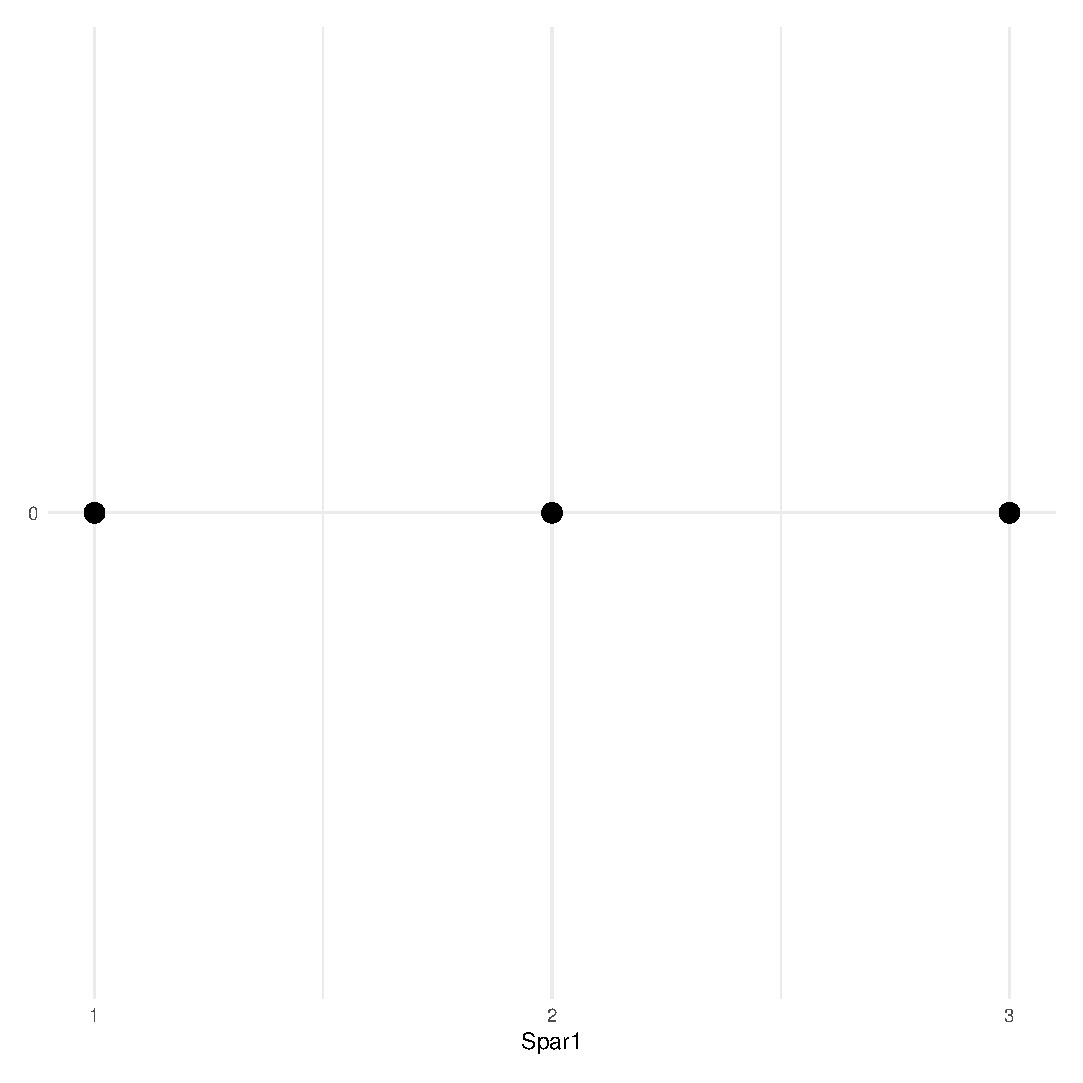
\includegraphics[width=0.6\textwidth]{../../images/points1}
  }
  \only<3>{%
    \centering
    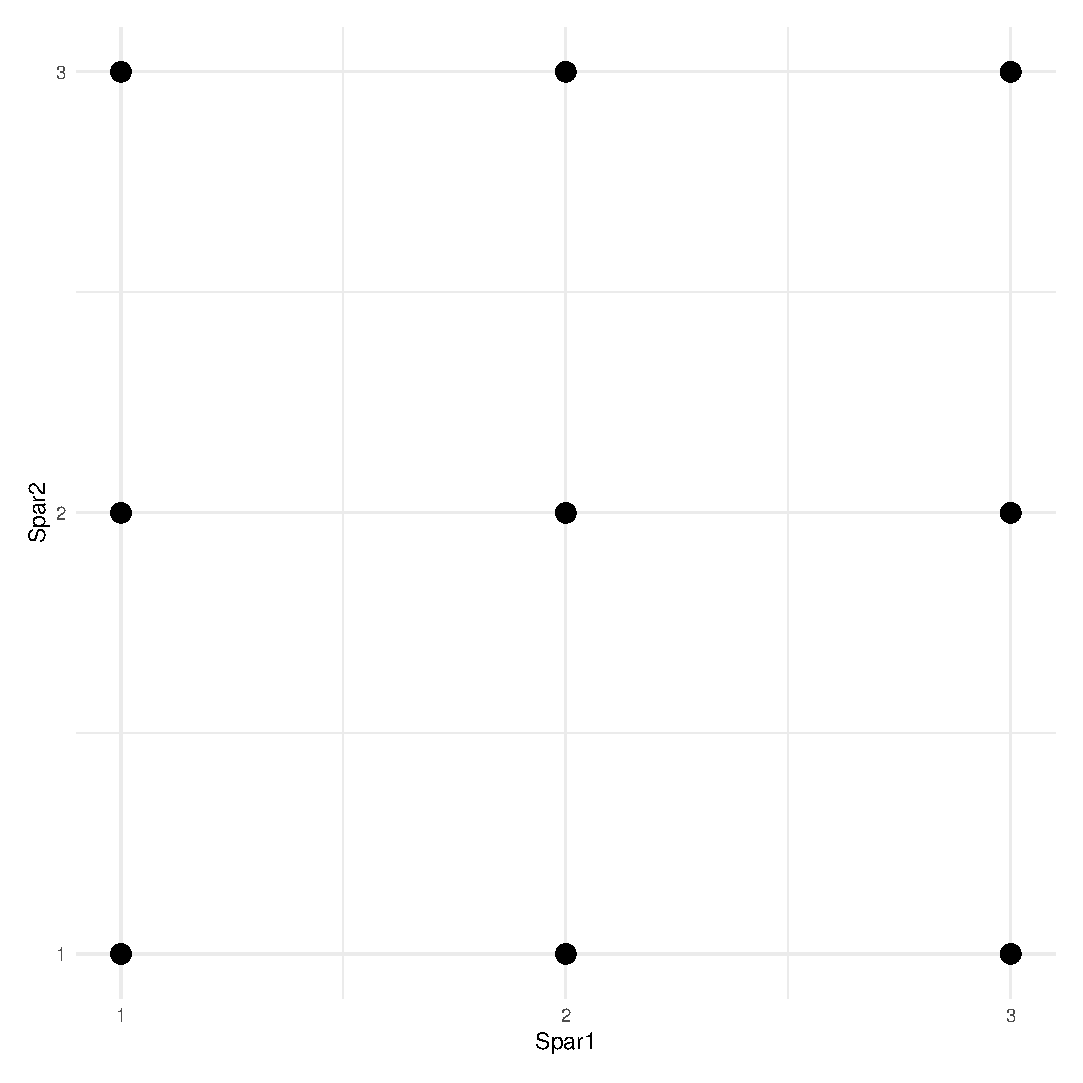
\includegraphics[width=0.6\textwidth]{../../images/points2}
  }
  \only<4>{%
    Scaling is \emph{exponential}, e.g.
    \begin{equation*}
      \text{Time} = (10\text{ seconds})^d
    \end{equation*}
  }
\end{frame}

% -------------------------
\begin{frame}{Computational Time}
  \visible<2>{\alert{The Curse of Dimensionality}}
  \begin{table}
    \begin{tabular}{r|r|l}
    \hline
    Dimension & Time (sec) & Comparison\\
    \hline
    1 & $10^{1}$ & Ten seconds\\
    \hline
    5 & $10^{5}$ & One Day\\
    \hline
    10 & $10^{10}$ & Eleven generations\\
    \hline
    18 & $10^{18}$ & Age of Universe\\
    \hline
    20 & $10^{20}$ & 230 x AoU\\
    \hline
    \end{tabular}
  \end{table}
\end{frame}

% -------------------------
%% \begin{frame}{UQ Tasks}
%%   High-dimensional integrals
%%   \begin{itemize}
%%   \item Moments $\E[\mX^n]$
%%   \item Probabilities $\E[\i1(\mX<x)]$
%%   \end{itemize}

%%   \bigskip Quadrature via full factorial (tensor grid) is exponential \\
%%   We need to address the Curse
%% \end{frame}

% -------------------------
\begin{frame}{Speaker Goals}
  \begin{itemize}
  \item Motivate
  \item Details and pointers
  \item New stuff
  \end{itemize}
\end{frame}

% -------------------------
\begin{frame}{Outline}
  \begin{outline}
  \1 UQ Tasks (Done)
  \1 Curse of Dimensionality
    \2 High-dimensional geometry
  \1 Lifting the Curse
    \2 Dimension reduction
    \2 Intrinsic dimensionality
  \end{outline}
\end{frame}

% --------------------------------------------------
%% SEC: Curse of Dimensionality
% --------------------------------------------------
\begin{frame}{Background}
  \begin{outline}
  \1 ``Curse of Dimensionality'' -- Richard Bellman (1961) \\
  \1 \emph{Vague} term
    \2 Integration
    \2 Sampling
    \2 Machine Learning
    \2 Inference
    \2 Distance
    \2 Big data
  \end{outline}
\end{frame}

% -------------------------
\framecard{\centering
``The trend today is towards more observations \emph{but even more so},
\alert{to radically larger numbers of variables} – voracious, automatic,
systematic collection of hyper-informative detail about each observed
instance.''

\bigskip
-- David Donoho, 2000\\
\tiny (Emphasis added)
}

% -------------------------
\begin{frame}{My Point}
  Curse of Dimensionality is \emph{everywhere} \\
  Lots of \emph{very different} perspectives

  \bigskip
  So what's up with high dimensions?
\end{frame}

% -------------------------
\framecard{\huge\centering%
      Weird facts about\\
      High-Dimensional\\
      Geometry
}

% -------------------------
\begin{frame}{Fact 1}
  The hypersphere has vanishing interior
\end{frame}

% -------------------------
\begin{frame}{Unit Hypersphere Volume}
  \begin{equation*} \begin{aligned}
      HV &= \int\cdots\int \alert{r^{d-1}}\,
           T(\varphi_{1},\dots,\varphi_{d-1})\,
           dr d\varphi_{1}\cdots d\varphi_{d-1}
  \end{aligned} \end{equation*}
\end{frame}

% -------------------------
\framepich{../../images/surface_density}{}

% -------------------------
\begin{frame}{Fact 2}
  The hypersphere concentrates at \emph{the} equator
\end{frame}

% -------------------------
\framepich{../../images/great_circle}{}

% -------------------------
\begin{frame}{A Wordgame}
  \emph{An} equator is always $d-1$ dimensional \\

  \bigskip An epsilon-band around a great circle can be made to hold an
  arbitrary volume-fraction
\end{frame}

% -------------------------
\framepich{../../images/equator}{}

% -------------------------
\begin{frame}{Fact 3}
  Johnson-Lindenstrauss Lemma:

  \bigskip \emph{Random projections} preserve \\
  \emph{pairwise distances}
\end{frame}

% JL: Example
% -------------------------
\begin{frame}[fragile]{JL: Example}
Example: Gene expression levels for some tumor types

\bigskip
  \begin{lstlisting}
## Gene data from UCI
dim(gene_data)
#       Obs,  Dim
> [1]   801 20531
  \end{lstlisting}

  \bigskip
  Note: This code on GitHub: https://github.com/zdelrosario/hyperspace
\end{frame}

% -------------------------
\begin{frame}[fragile]{JL: Example}
  \begin{lstlisting}
eps <- 0.1             # 10% distort
n <- dim(gene_data)[1] # Observations
d <- dim(gene_data)[2] # Dimension

k <-  2 * ceiling(C * log(n) / eps ^ 2)
k
# Intrinsic dimensionality
> 1338 (6.5% of 20531)
  \end{lstlisting}
\end{frame}

% -------------------------
\begin{frame}[fragile]{JL: Example}
  \begin{lstlisting}
## Randomly project
P_k <- random_projection(k x d)
## Project
projected_data = gene_data %*% P_k
## Match mean distances
a <- mean_distance(gene_data) /
  mean_distance(projected_data)
projected_data = a * projected_data
  \end{lstlisting}
\end{frame}

% -------------------------
\begin{frame}[fragile]{JL: Example}
  \begin{lstlisting}
eps
# Requested distortion
>    10%
quantile(relative_difference)
# Quantile
>      0%     25%    50%    75%   100%
# Realized distortion
> -7.784% -1.193% 0.082% 1.344% 8.139%
  \end{lstlisting}
\end{frame}

% -------------------------
\begin{frame}{Why Does This Work?}
  \underline{Claim}: For any $0<\epsilon<1$ and $n\in\mathbb{Z}_{>0}$, let
  $k\in\mathbb{Z}_{>0}$ such that

  \begin{equation*}
    k \geq C \frac{\log(n)}{\epsilon^2},
  \end{equation*}

  \noindent then for all sets of points $V\subset\R{d}$, there is a projection
  $P_k:\R{d}\to\R{k}$ such that, for all $u,v\in V$, we have

    \begin{equation*}
      \alert<2>{(1 - \epsilon)\|\vu - \vv\|^2 \leq \alpha\|P_k(\vu) - P_k(\vv)\|^2 \leq %
      (1 + \epsilon)\|\vu - \vv\|^2
}    \end{equation*}
\end{frame}

% JL: Distance
% -------------------------
\begin{frame}{}
    \begin{equation*} \begin{aligned}
        (1 - \epsilon)(\text{Distance})^2 &\leq %
          \alpha(\text{Projected Distance})^2 \\
        &\, \\
        \alpha(\text{Projected Distance})^2 &\leq %
          (1 + \epsilon)(\text{Distance})^2\\
    \end{aligned} \end{equation*}
\end{frame}

% JL: Projections
% -------------------------
\begin{frame}[t]{}
  % Content
  \begin{equation*}
    (1 - \epsilon)\|\vu - \vv\|^2 \leq %
    \alert{\alpha}\|P_{\alert{k}}(\vu) - P_{\alert{k}}(\vv)\|^2 \leq %
    (1 + \epsilon)\|\vu - \vv\|^2
  \end{equation*}
  % Annotation
  \visible<2->{%
    \begin{textblock}{6}(+5.0,+5.0)
      {\textblockcolor{}
        \centering%
        \only<2>{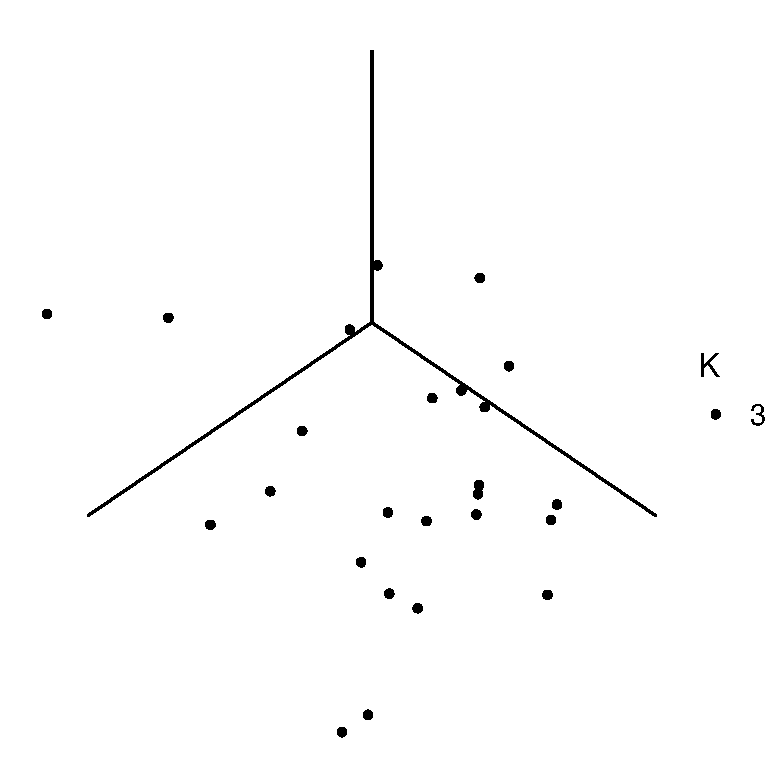
\includegraphics[width=1.0\textwidth]{../../images/dim_proj3}}
        \only<3>{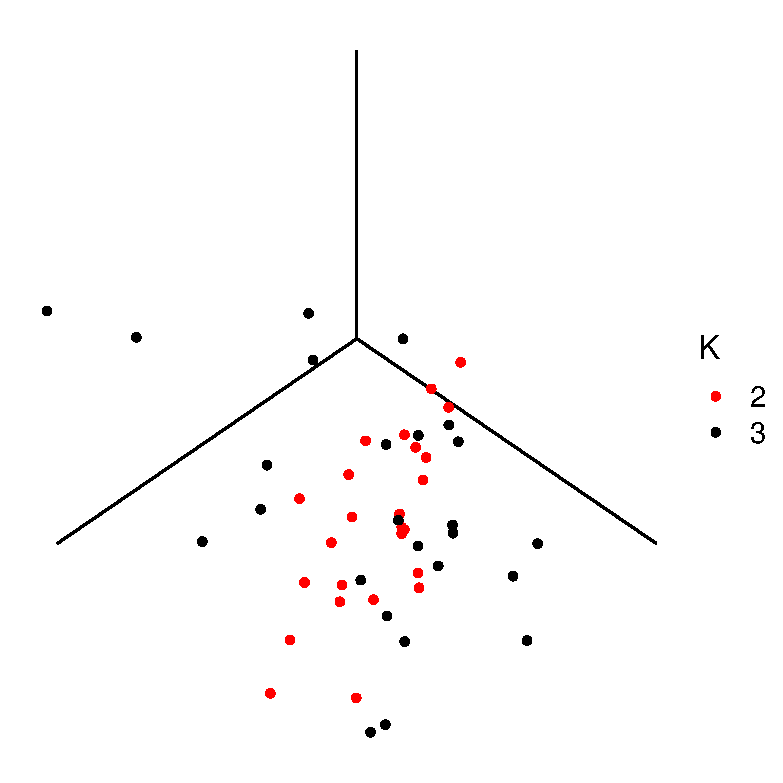
\includegraphics[width=1.0\textwidth]{../../images/dim_proj2}}
        \only<4>{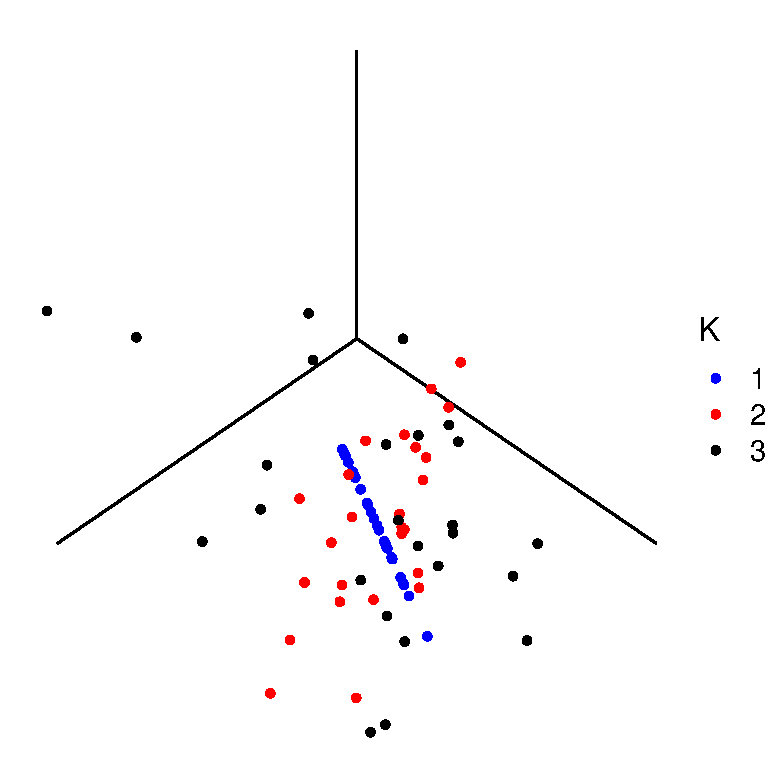
\includegraphics[width=1.0\textwidth]{../../images/dim_proj1}}
      }
    \end{textblock}
  }
\end{frame}

% JL: Dimensionality
% -------------------------
\begin{frame}{}
  % Content
  \begin{equation*}
    \alert<2>{k} \geq C\frac{\log(\alert<3>{n})}{\alert<4>{\epsilon}^2}
  \end{equation*}
  % Annotation
  \only<2->{%
    \begin{textblock}{4}(+0.5,+0.5)
      {\textblockcolor{}
        $k$ is the projection dimension
      }
    \end{textblock}
  }
  \only<3->{%
    \begin{textblock}{4}(+0.5,+11.0)
      {\textblockcolor{}
        $n$ is the number of observations
      }
    \end{textblock}
  }
  \only<4->{%
    \begin{textblock}{4}(+11.0,+11.0)
      {\textblockcolor{}
        $\epsilon$ is the desired error
      }
    \end{textblock}
  }
  \only<5->{%
    \begin{textblock}{5.0}(+11.0,+0.5)
      {\textblockcolor{}
        Dimensionality is\\
        \emph{curiously absent!}
      }
    \end{textblock}
  }
  \only<6>{%
    \begin{textblock}{4.5}(+5.5,+8.0)
      {\textblockcolor{}
        $k$ is an \emph{intrinsic dimensionality}
      }
    \end{textblock}
  }
\end{frame}

% --------------------------------------------------
%% SEC: Dimension Reduction
% --------------------------------------------------
\framecard{\huge\centering%
  Dimension Reduction
}

% -------------------------
\begin{frame}{Dimension Reduction}
  Idea: Identify low-dimensional structure; \\
  reduce effective dimension

  \bigskip If $\text{Cost} = C^d$, \\
  greatest payoff is reducing $d$
\end{frame}

% -------------------------
\begin{frame}{Dimension Reduction \textcolor{palegreen}{In UQ}}
  \bigskip \textcolor{palegreen}{J-L showed us \emph{linear} low-dimensional structure} \\
  \textcolor{palered}{J-L does not separate \emph{inputs} and \emph{response}}

  \bigskip We've talked about $\vx$ \\
  What about $f(\vx)$?
\end{frame}

% -------------------------
\begin{frame}{DR Taxonomy}
  \begin{outline}
  \1 Generic-space DR (J-L, PCA, etc.)
    \2 No additional structure on $\R{d}$
  \1 Output-space DR (ROMs, CS, etc.)
    \2 $\R{d}$ is state space, often temporal structure
  \1 \alert<2>{Input-space DR} (CS, ...)
    \2 $\R{d}$ is input space, connected to response
  \end{outline}
\end{frame}

% -------------------------
\begin{frame}{Running Example: Pipe Flow}
  \centering
  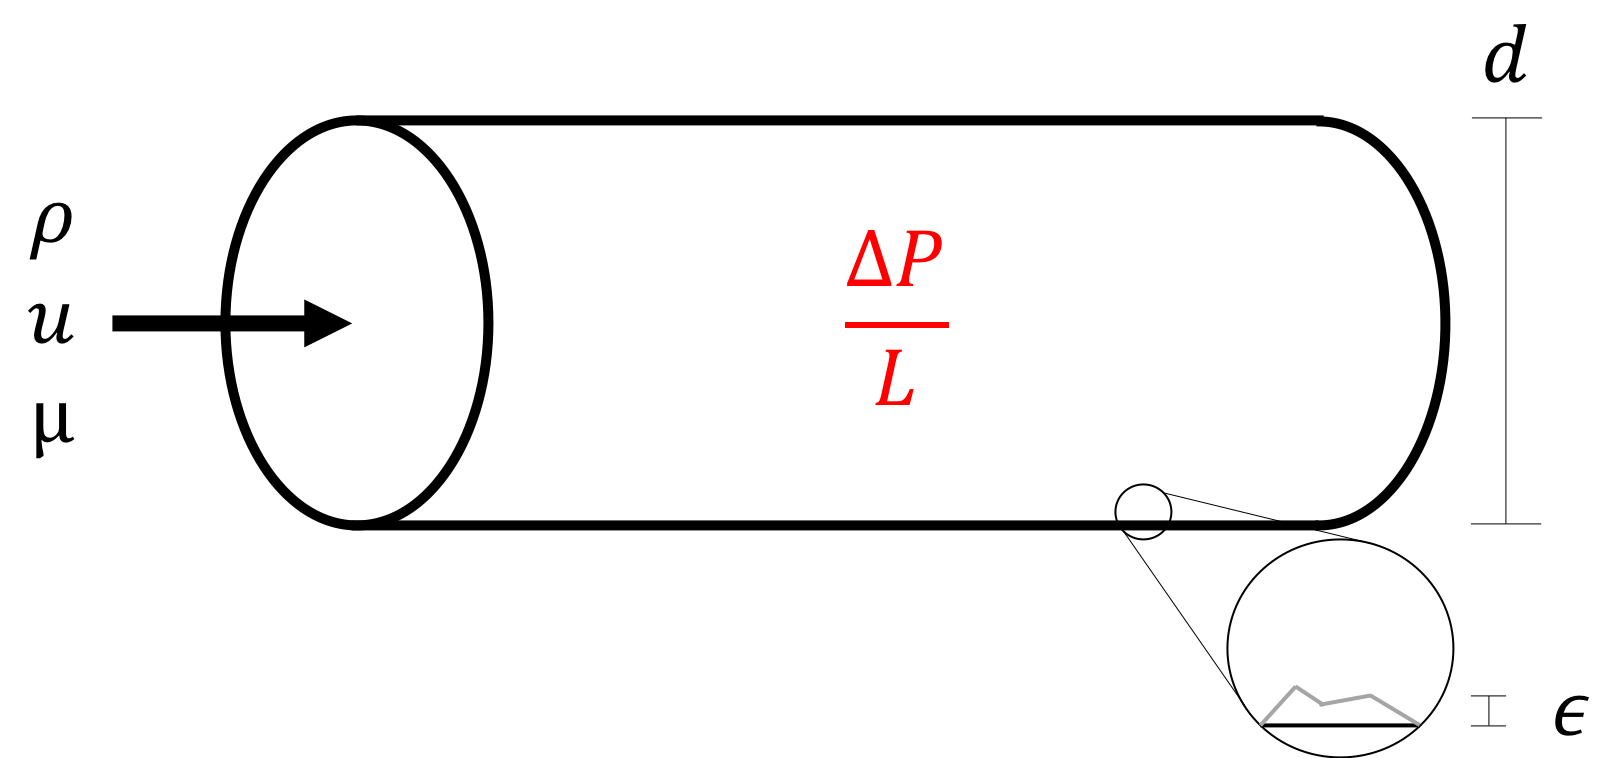
\includegraphics[width=0.9\textwidth]{../../images/pipe_diagram}

  \begin{textblock}{6.0}(+0.5,+11.0)
    \visible<2>
      {\textblockcolor{}
        qoi: (normalized) pressure loss \\
        inputs: $\rho, u, d, \mu, \epsilon$
      }
  \end{textblock}
\end{frame}

% -------------------------
\begin{frame}{Dimension Reduction: Methods}
  \begin{outline}
    \1 Subset reduction
      \2 Morris screening
      \2 Sobol' indices
    \1 Subspace reduction
      \2 PCA-primer
      \2 Active subspaces
  \end{outline}
\end{frame}

% -------------------------
\begin{frame}{Subset Reduction}
  Suppose $\vx^{\top} = [\vx_A^{\top}, \vx_I^{\top}]$ \\
  What if some variables were \emph{inactive}? E.g.

  \begin{equation*}
    f(\vx_A, \vx_I) = f(\vx_A, \vx'_I),
  \end{equation*}

  \noindent for all $\vx_A$ and $\vx_I \neq \vx'_I$. \\
  Can then \emph{ignore} $\vx_I$.
\end{frame}

% -------------------------
\begin{frame}{Subset Reduction: Methods}
  \begin{outline}
    \1 Morris screening
      \2 \textcolor{palegreen}{Inexpensive}
      \2 \textcolor{palered}{Difficult to interpret}
    \1 Sobol' indices
      \2 \textcolor{palegreen}{Clear interpretation}
      \2 \textcolor{palered}{Can be expensive}
  \end{outline}
\end{frame}

% -------------------------
\begin{frame}{Sobol' Indices}
  Idea: Attribute \emph{variance in output} $f$ \\
  to \emph{different inputs}

  \bigskip E.g.
  \begin{table}
    \centering
    \begin{tabular}{@{}llllll@{}}
     & $\rho$ & $U$ & $d$ & $\mu$ & $\epsilon$\\
    \hline
    $\V[f]$ & 0\% & 0\% & 6\% & 0\% & 94\% \\
    \end{tabular}
  \end{table}

  \visible<2>{\alert{How to \emph{attribute} variance?}}
\end{frame}

% -------------------------
\begin{frame}{Sobol' Formulation}
  Variance decomposition
  \begin{equation*}
    \V[Y] = \E[\V[Y|\mX_{\vu}]] + \V[\E[Y|\mX_{\vu}]]
  \end{equation*}

  Notation: \\
  Ex. $\vu = \{\rho,u,d,\mu\}$ \\
  $-\{\epsilon\} = \{\rho,u,d,\mu\}$
\end{frame}

% -------------------------
\begin{frame}{First-order Index}
   First-order index
  \begin{equation*}
    \underline{\tau}_{\{i\}}^2 = \frac{\alert<3>{\V[\alert<2>{\E[Y|X_i]}]}}{\V[Y]}
  \end{equation*}

  % Annotation
  \visible<2->{Average over \emph{all but} $X_i$\\}
  \visible<3>{Variance due to $X_i$ \emph{alone}}
\end{frame}

% -------------------------
\begin{frame}{Total-order Index}
  Total-order index
  \begin{equation*}
    \overline{\tau}_{\{i\}}^2 = \frac{\alert<3>{\E[\alert<2>{\V[Y|X_{-\{i\}}]}]}}{\V[Y]}
  \end{equation*}

  % Annotation
  \visible<2->{Variance due to \emph{only} $X_i$\\}
  \visible<3>{\emph{Average variance} due to $X_i$ \emph{with interactions}}
\end{frame}

% -------------------------
\begin{frame}{Sobol' Elaboration}
  \begin{equation*} \begin{aligned}
      \text{First} &\leq \text{Total} \\
      0 \leq \underline{\tau}_{\{i\}}^2 &\leq \overline{\tau}_{\{i\}}^2 \leq 1
  \end{aligned} \end{equation*}
\end{frame}

% -------------------------
\begin{frame}{Sobol' Example}
  \begin{equation*} \begin{aligned}
    f(\vx) &= \sin(x_1) + 7\sin^2(x_2) + 0.1 \alert<2->{x_3^4\sin(x_1)} \\
    x_1, x_2, x_3 &\sim U[-\pi, \pi], \\
    \alert<2>{\underline{\tau}_{\{3\}}^2} &= \alert<2>{0\%}, \\
    \alert<3>{\overline{\tau}_{\{3\}}^2} &= \alert<3>{24.4\%}
  \end{aligned} \end{equation*}

  \visible<2->{Input 3 has no main effect}\\
  \visible<3>{\emph{But} input 3 has an interaction}\\
  \footnotetext{\tiny Ishigami \& Homma (1990)}
\end{frame}

% -------------------------
\begin{frame}{But wait...}
  Sobol' indices based on \emph{variance}... \\
  Variance is an \emph{expectation}... \\
  Expectations are \emph{cursed by dimensionality}...

  \bigskip Sobol' is cursed by dimensionality! \\
\end{frame}

% -------------------------
\begin{frame}{Using Sobol'}
  Formulated for analytic models

  \bigskip Surrogate models can extend functionality
\end{frame}

% -------------------------
\begin{frame}{Intrinsic Dimensionality}
  Idea: Find a method whose computational cost scales with \emph{intrinsic
    dimensionality} $k$,\\ \alert{not} dimensionality $d$....
\end{frame}

% -------------------------
\begin{frame}{Subspace Reduction: Methods}
  \begin{outline}
    \1 Principal Component Analysis (PCA)
      \2 Intuition
    \1 Active subspaces
      \2 Application
  \end{outline}
\end{frame}

% -------------------------
\begin{frame}{Principal Component Analysis}
  \huge\underline{Idea:} Find directions that capture variability
\end{frame}

% -------------------------
\framepich{../../images/pca1}{}
\framepich{../../images/pca2}{}
\framepich{../../images/pca3}{
  \begin{textblock}{7}(+9.0,+10.0)
    \visible<2>{
      {\textblockcolor{}
        Direction \alert{from data} \\
        Called \emph{principal component analysis}
      }
    }
  \end{textblock}
}

% -------------------------
\begin{frame}{PCA Formalism}
  Given zero-mean data $\mX\in\R{n\times d}$

  \begin{equation*}
    \mX = \mU\m\Sigma\mV^{\top}
  \end{equation*}

  \noindent with ordered $\sigma_1\geq\dots\geq\sigma_r\geq0$\\
  standard deviations \\

  Select $k \leq d$, project on first $k$ directions, gives new variables
  $\mY\in\R{n\times k}$

  \begin{equation*}
    \mY = \mX\mV_k = \mU\m\Sigma_k
  \end{equation*}

  Often $k$ selected to capture a fraction of the variance
\end{frame}

% -------------------------
\begin{frame}{PCA For Models}
  PCA is for Generic-spaces \\
  How to handle Input-spaces?

  \bigskip Idea: Do a PCA on \emph{gradient data}
\end{frame}

% -------------------------
\framepich{../../images/as_contour0}{}
\framepich{../../images/as_contour1}{}

% -------------------------
\begin{frame}{Active Subspace}
  \begin{equation*} \begin{aligned}
      \mC &= \E[\nabla_{\vx}f\nabla_{\vx}f^{\top}] \\
          &= \mU\m\Sigma\mV^{\top} \\
          &\approx \frac{1}{n}\sum_{i=1}^n \nabla_{\vx}f_i\nabla_{\vx}f^{\top}_i \\
          &= \hat{\mU}\hat{\m\Sigma}\hat{\mV}^{\top}
  \end{aligned} \end{equation*}

  \footnotetext{\tiny Constantine (2015)}
\end{frame}

% -------------------------
\begin{frame}{AS Selecting $k$}
  Standard arguments bound subspace error based on \emph{eigenvalue gap} $\delta
  = \sigma_{j+1} - \sigma_j$

  \begin{equation*}
    \|\sin(\m\Theta_0)\| \leq \frac{\|\mR\|}{\delta}
  \end{equation*}

  For the pipe flow example
  \begin{table}
    \centering
    \begin{tabular}{@{}ll@{}}
      \hline
      Gap Fraction & Dimension\\
      \hline
      0.9892887 & 1\\
      \hline
      0.0053363 & 2\\
      \hline
      0.0000129 & 3\\
      \hline
      0.0000000 & 4\\
      \hline
    \end{tabular}
  \end{table}

  \footnotetext{\tiny Davis \& Kahan (1970)}
\end{frame}

% -------------------------
\begin{frame}{Using the AS}
  \begin{equation*} \begin{aligned}
      \vx_A &= \mV_A^{\top}\vx \\
      \vx_I &= \mV_I^{\top}\vx
  \end{aligned} \end{equation*}

  \begin{figure}
    \centering
    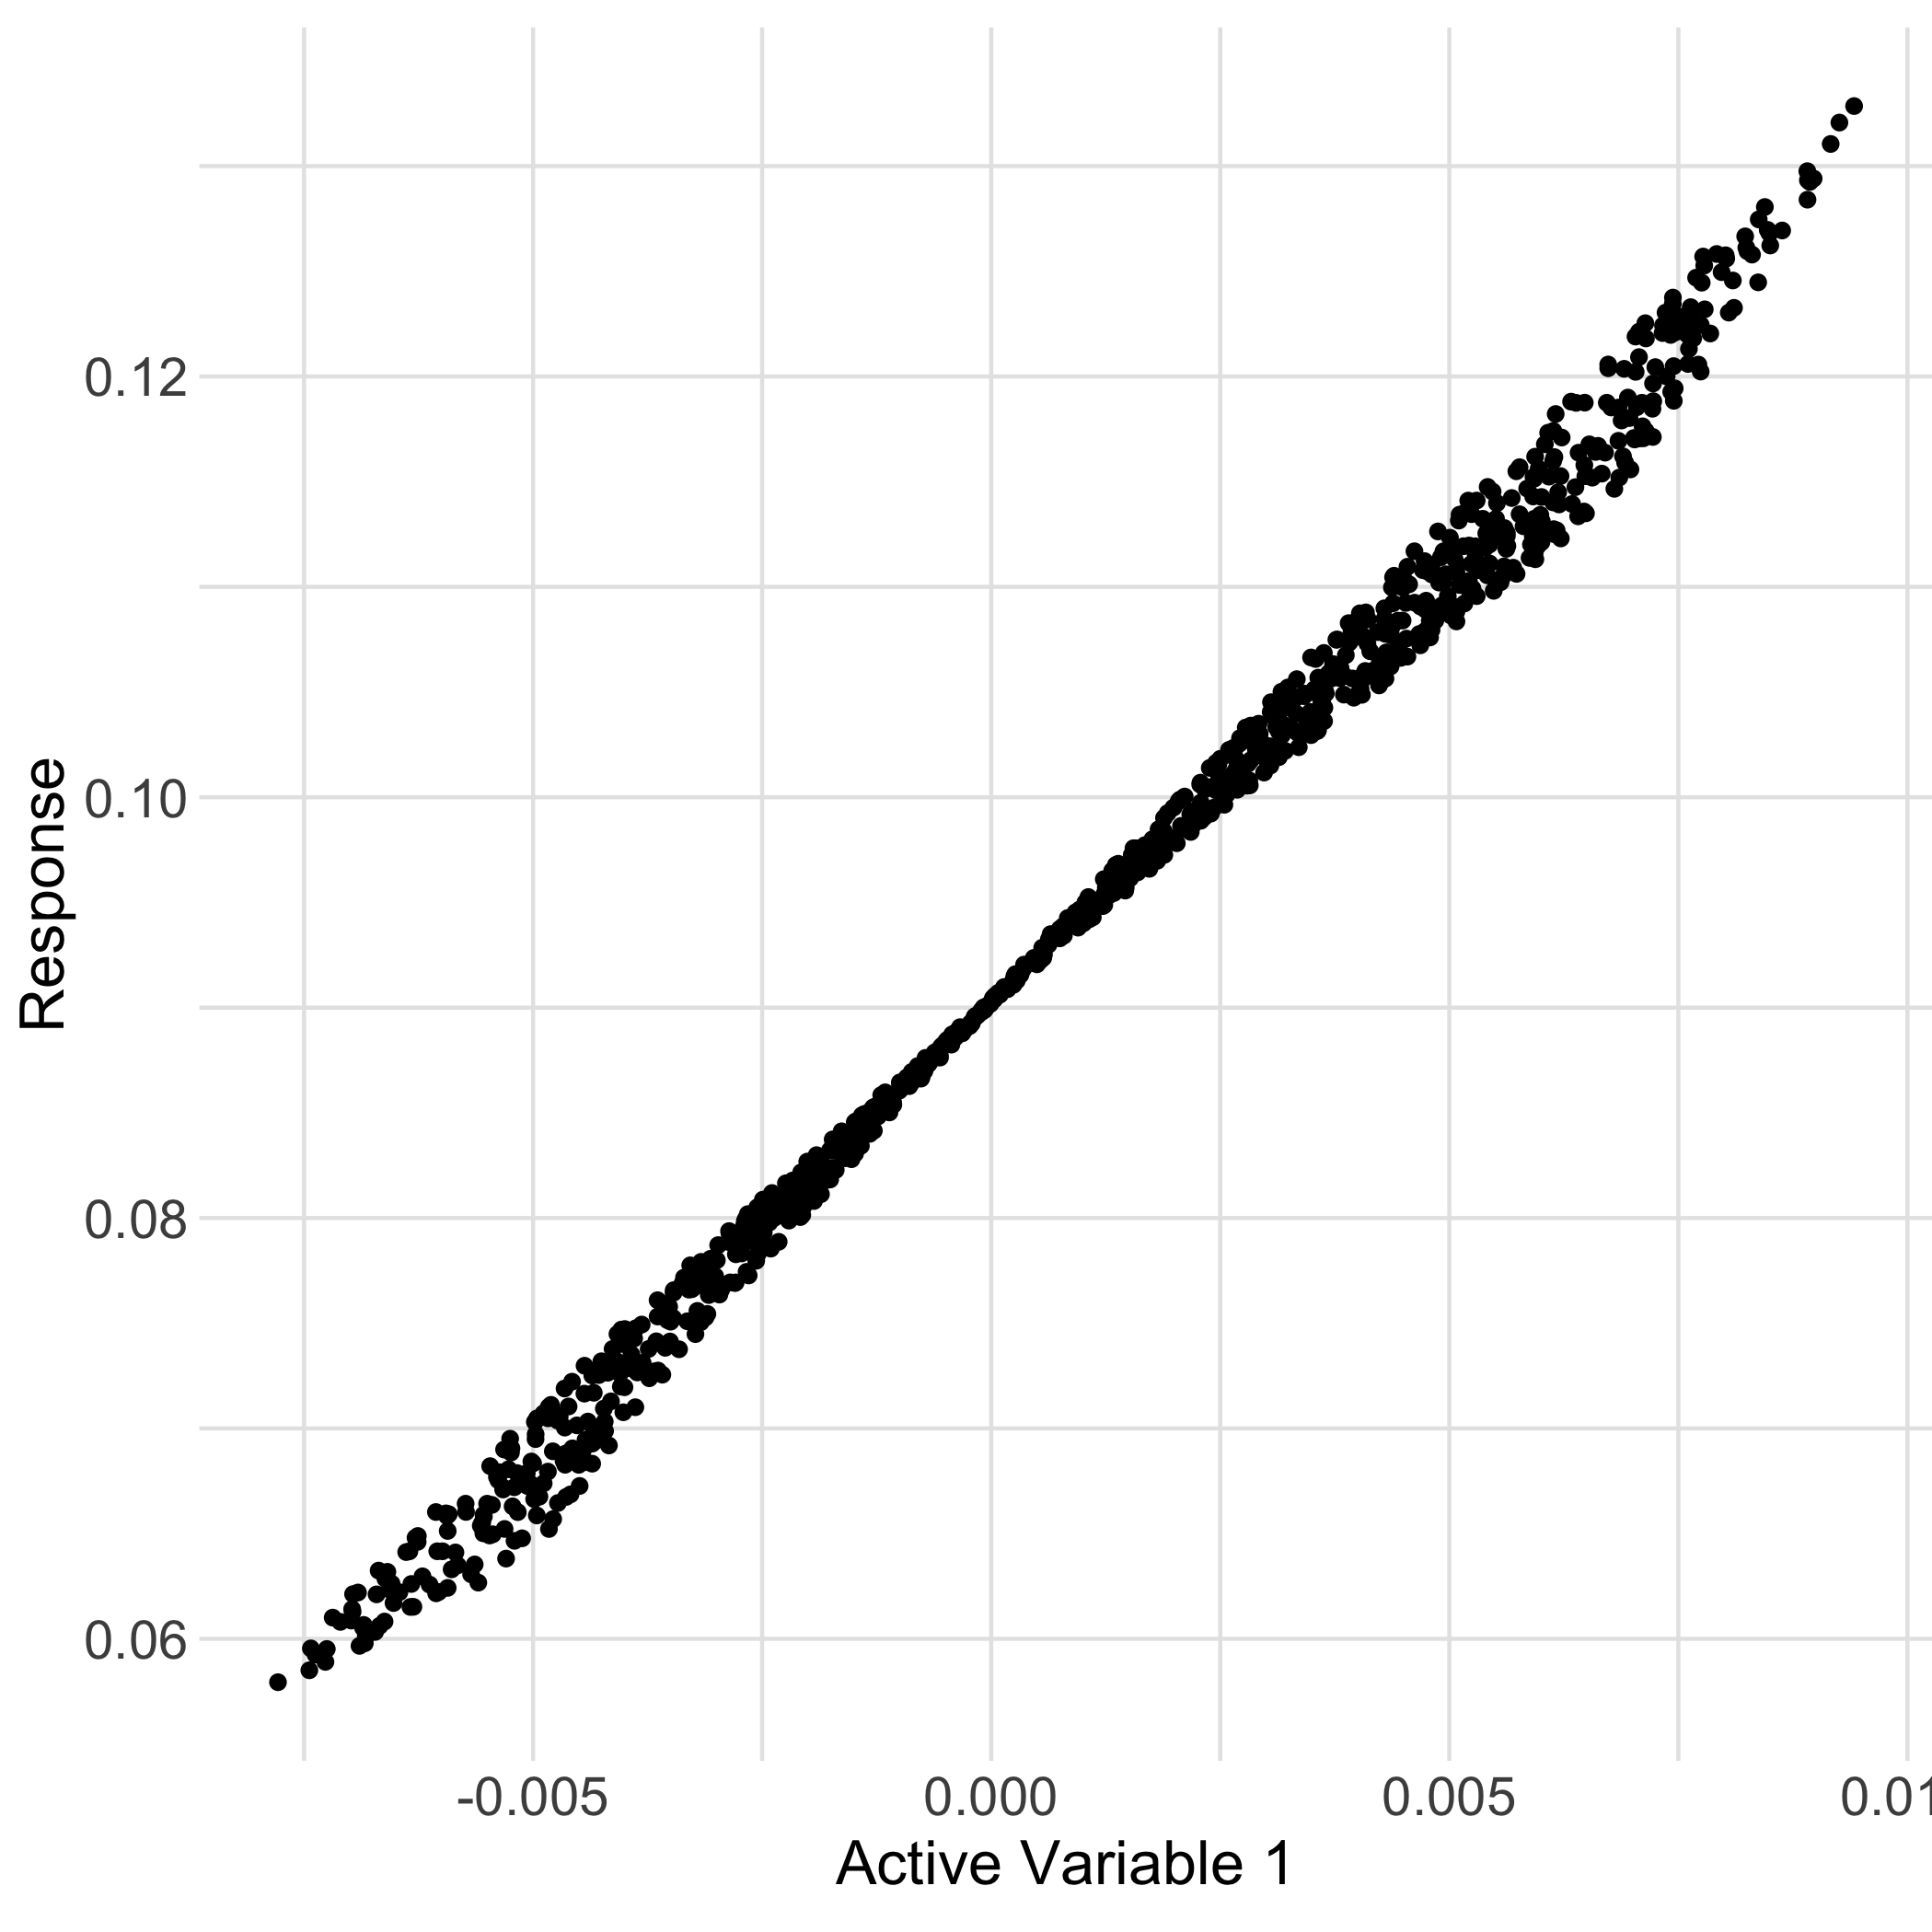
\includegraphics[width=0.5\textwidth]{../../images/as_summary_nat}
  \end{figure}
\end{frame}

% -------------------------
\begin{frame}{But Wait...}
  The active subspace matrix $\mC$ is defined via expectation

  \bigskip It is cursed by dimensionality?
\end{frame}

% -------------------------
\begin{frame}{AS Intrinsic Dimensionality}
  \begin{equation*}
    n \geq \frac{C}{\epsilon^2}\log\left(\frac{4}{p}\text{intdim}(\mC)\right)
  \end{equation*}

  where

  \begin{table}
    \centering
    \begin{tabular}{@{}ll@{}}
      $n$ & Required samples \\
      $\epsilon$ & Desired error tolerance \\
      $p$ & Probability of failure
    \end{tabular}
  \end{table}

  and

  \begin{equation*}
    \text{intdim}(\mC) = \frac{\text{trace}(\mC)}{\|\mC\|_2} \geq 1
  \end{equation*}

  \footnotetext{\tiny Holodnak, Ipsen, and Smith (2018)}
\end{frame}

% -------------------------
\begin{frame}{Intrinsic Dimensionality}
  \huge Where does \emph{intrinsic dimensionality} come from?
\end{frame}

% -------------------------
\begin{frame}{Related Concepts}
  \begin{itemize}
  \item \textbf{Sparsity} -- Compressed sensing
  \item \textbf{Low-rank} -- Linear algebra
  \item \textbf{Dimensionality} -- Dimension reduction
  \visible<2>{\item \textbf{Pi groups} -- Dimensional analysis}
  \end{itemize}
\end{frame}

% -------------------------
\begin{frame}{Dimensional Analysis}
  Buckingham pi

  \begin{equation*} \begin{aligned}
      \pi &= f(\vz) \\
          &= \psi(\pi_1,\dots,\pi_{d-r})
  \end{aligned} \end{equation*}

  where

  \begin{equation}
    \pi_i = \prod_{j=1}^d z_j^{w_{ij}}
  \end{equation}

  \footnotetext{\tiny Buckingham (1914)}
\end{frame}

% -------------------------
\begin{frame}{Dimensional Analysis}
  \alert{Modified}\footnote{del Rosario et al. (2017)} Buckingham pi

  \begin{equation*} \begin{aligned}
      \pi &= f(\vz) \\
          &= \psi'(\mW^{\top}\vx)
  \end{aligned} \end{equation*}

  where $\vx = \log(\vz)$ and

  \begin{equation}
    \mD\mW = 0
  \end{equation}
\end{frame}

% -------------------------
\begin{frame}{DA Example}
  \begin{table}
    \begin{tabular}{@{}lccccc@{}}
      \toprule
      Dimension  & $\rho$ & $u$   & $d$ &  $\mu$ & $\epsilon$\\
      \midrule
      Mass (M)   &   1    &  0    &  0  &    1   &  0 \\
      Length (L) & \mm3   &  1    &  1  &  \mm1  &  1 \\
      Time (T)   &   0    & \mm1  &  0  &  \mm1  &  0 \\
      \bottomrule
      $Re$       &   1    &  1    &  1  &  \mm1  &  0 \\
      $R$        &   0    &  0    & \mm1&    0   &  1
    \end{tabular}
  \end{table}

  \visible{\bigskip Dimensionality $5$\\ Intrinsic dimensionality $2$}
\end{frame}

% -------------------------
\begin{frame}{Pi Subspace}
  Active subspace $\subseteq$ \emph{Pi subspace} $\cR(\mW)$

  \bigskip The pi subspace is \emph{a priori bound on dimensionality}

  \bigskip Intuitive notion of intrinsic dimensionality
\end{frame}

% -------------------------
\begin{frame}{Pi Subspace Example}
  \begin{figure}
    \centering
    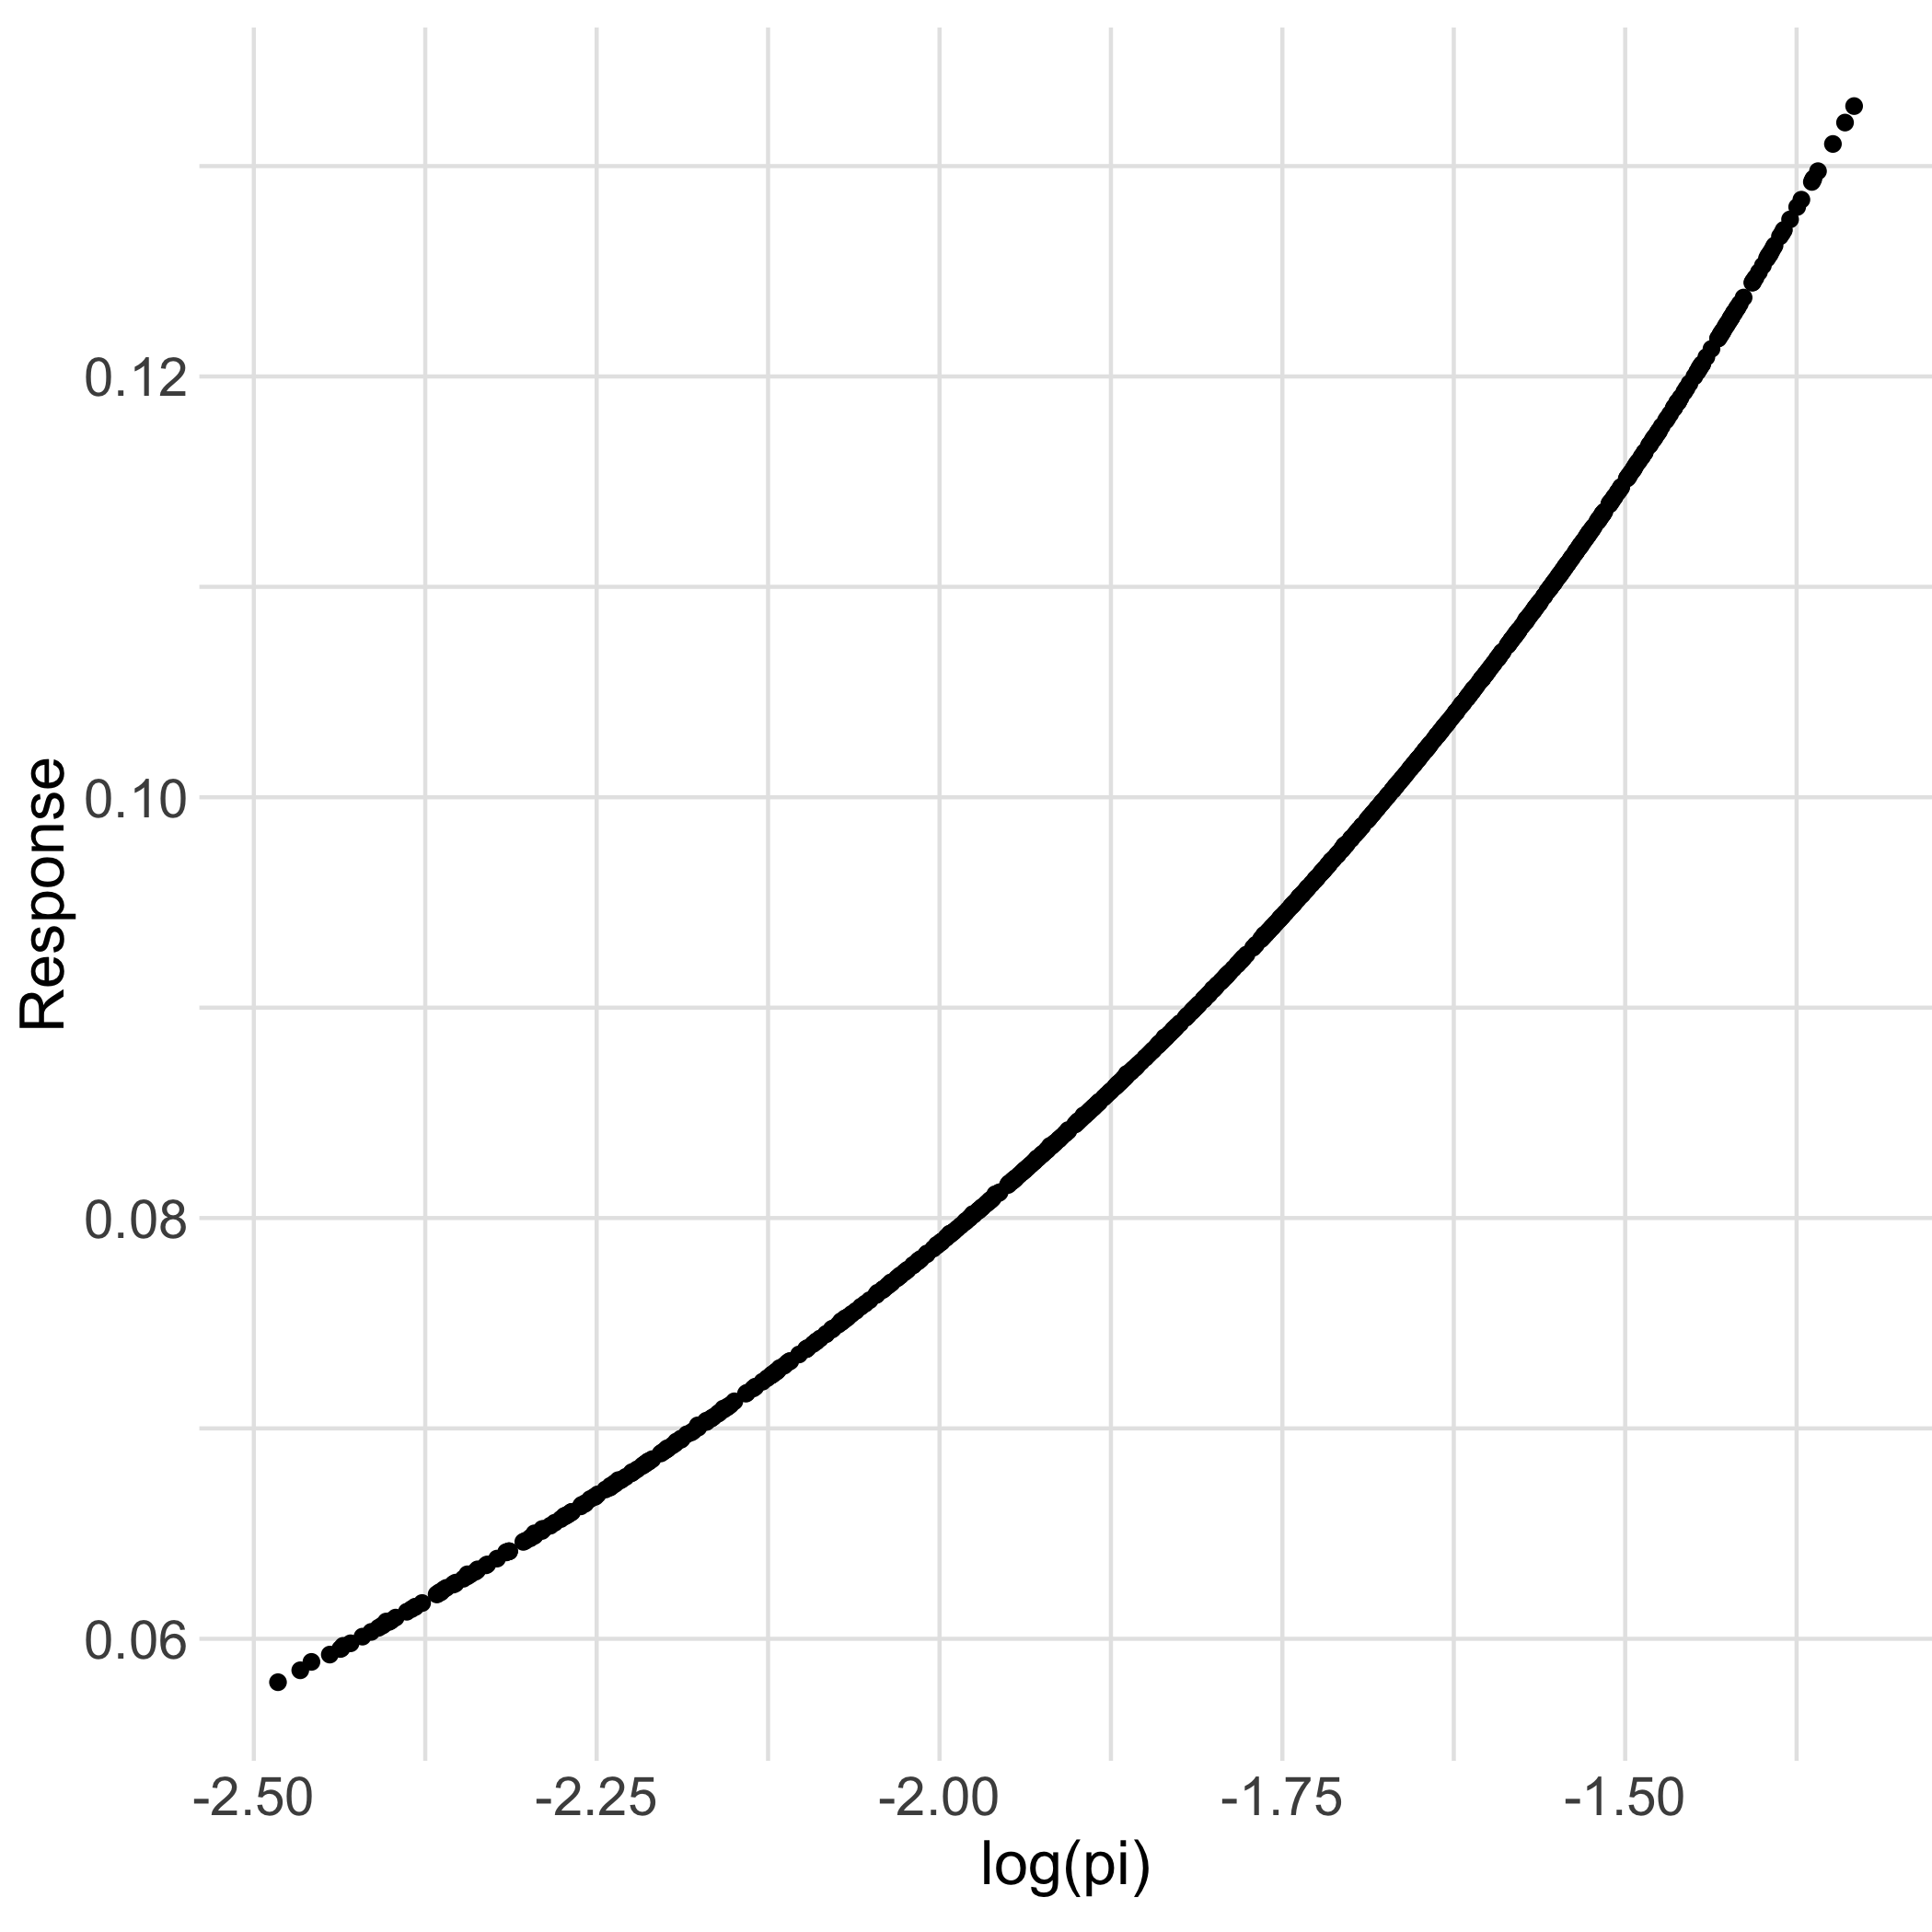
\includegraphics[width=0.7\textwidth]{../../images/as_summary_pi}
  \end{figure}

  % Annotate
  \begin{textblock}{7}(+6.0,+12.7)
    \visible<2>{%
      \begin{tabular}{@{}llllll@{}}
                & $\rho$ & $u$  & $d$   & $\mu$ & $\epsilon$ \\
        $\vw_1$ & 0.00   & 0.00 & -0.71 & 0.00  & 0.71
      \end{tabular}
    }
  \end{textblock}
\end{frame}

% -------------------------
\begin{frame}{Other Uses}
  \emph{Physically relevant} notion of intrinsic dimensionality has other uses:

  \begin{itemize}
  \item Identify \emph{unique and relevant} dimensionless numbers\footnote{Constantine et al. (2017)}
  \item Detect \emph{lurking variables}\footnote{del Rosario et al. (2017)}
  \item Constrained machine learning (Forthcoming...)
  \end{itemize}
\end{frame}

% -------------------------
\framecard{\huge\centering%
  Concluding thoughts
}

% -------------------------
\begin{frame}{The Curse of Dimensionality}
  \begin{itemize}
  \item Is everywhere
  \item Is exponential
  \item Motivates \emph{dimension reduction}
  \end{itemize}
\end{frame}

% -------------------------
\begin{frame}{Dimension Reduction}
  \begin{itemize}
  \item Finds low-dimensional structure
  \item Is tailored to different spaces
  \item Often scales with \emph{intrinsic dimensionality}
  \end{itemize}
\end{frame}

% -------------------------
\begin{frame}{Intrinsic Dimensionality}
  \begin{itemize}
  \item Is problem-dependent
  \item Enables deeper insights
  \item Is waiting to be discovered!
  \end{itemize}

  \bigskip\centering zdr@stanford.edu
\end{frame}

\end{document}
